\documentclass[11pt,letterpaper]{article}
\usepackage{../assets/scientific_report}
\usepackage[brazil]{babel}
\usepackage{amsmath,float,listings,xcolor,graphicx,geometry}
\geometry{headheight=23pt,top=2cm,bottom=2cm,left=2.5cm,right=2.5cm}
\setlength{\parskip}{0.5em}\setlength{\parindent}{0pt}
\lstset{language=C,basicstyle=\ttfamily\small,keywordstyle=\color{blue}\bfseries,commentstyle=\color{green!60!black}\itshape,stringstyle=\color{red!80!black},numbers=left,numberstyle=\tiny\color{gray},numbersep=8pt,frame=single,breaklines=true,captionpos=b,tabsize=4,showstringspaces=false}
\begin{document}
\pagestyle{plain}
\begin{center}
{\LARGE\bfseries Escalabilidade da difusão viscosa no NPAD}\\[0.4em]
{\normalsize Eugenio Vitor Lopes dos Santos}\\[0.3em]
{\small DCA3703, Programação Paralela, Universidade Federal do Rio Grande do Norte}
\end{center}

\section{Enunciado}
\begin{quote}
Avaliar a escalabilidade do código de Navier--Stokes em um nó do NPAD. Identificar gargalos e comparar implementações otimizadas, discutindo escalabilidade geral, fraca e forte.
\end{quote}

\section{Fundamentação teórica}
A equação $\partial u/\partial t=\nu\nabla^2u$ é discretizada por Euler explícito e diferenças centrais, formando o stencil de cinco pontos:
\[
u^{k+1}_{i,j}=u^k_{i,j}+r(u^k_{i-1,j}+u^k_{i+1,j}+u^k_{i,j-1}+u^k_{i,j+1}-4u^k_{i,j}),
\qquad r=\nu\Delta t/h^2.
\]
Com $\nu=0{,}1$, $\Delta t=0{,}2$ e $h=1$, obtém-se $r=0{,}02$, dentro do limite de estabilidade bidimensional. Dois campos em \texttt{double} separam leitura e escrita. As bordas ficam fixas. Os campos nulo e constante devem permanecer invariantes, enquanto a perturbação gaussiana se difunde.

\subsection{Distribuição e sincronização}
O escalonamento \texttt{static} distribui blocos contíguos de linhas, adequado ao custo uniforme das células, em região paralela única nos 500 passos. Cada passo depende do anterior (RAW) e exige barreira após o stencil; a troca em \texttt{single} acrescenta segunda barreira, e ponteiros privados reduzem a troca a operação local. O bloco conservado por thread favorece a localidade temporal; o laço interno em j contíguo favorece a espacial.

\subsection{SIMD e inicialização paralela}
A diretiva \texttt{omp simd} sugere o processamento vetorial do laço interno, mas o compilador pode vetorizar sozinho, sem garantia de ganho. A inicialização paralela distribui a escrita dos dois campos; sob \textit{first touch} em NUMA, cada página se aproxima da thread que a escreveu primeiro.

\subsection{Indicadores de escalabilidade}
Para trabalho fixo $W$, o speedup e a eficiência são
\[
S(p,W)=\frac{T(1,W)}{T(p,W)},\qquad E(p,W)=\frac{S(p,W)}{p}.
\]
\begin{itemize}
\item \textbf{Desempenho.} Tempo de execução da aplicação.
\item \textbf{Eficiência.} Trabalho realizado com os recursos disponíveis para a execução.
\item \textbf{Escalabilidade.} Capacidade de obter melhor desempenho à medida que mais recursos computacionais são utilizados.
\item \textbf{Lei de Amdahl.} A parte do código que permanece sequencial limita o speedup máximo, por mais recursos que se adicionem.
\item \textbf{Lei de Gustafson.} Quando o problema cresce com a quantidade de processadores, a aplicação pode continuar apresentando ganhos significativos.
\item \textbf{Speedup.} Razão entre o tempo da referência e o tempo paralelo. Neste trabalho a referência é a própria estratégia com uma thread, pois o job não inclui versão sequencial.
\item \textbf{Escalabilidade forte.} Problema fixo, com aumento apenas do número de processadores.
\item \textbf{Escalabilidade fraca.} O problema cresce proporcionalmente aos processadores, mantendo aproximadamente a mesma carga por processador.
\item \textbf{Fortemente escalável.} Mantém a eficiência ao aumentar os recursos sem aumentar o problema.
\item \textbf{Fracamente escalável.} Mantém a eficiência quando o problema cresce menos que os recursos.
\end{itemize}
O tempo paralelo soma a parcela útil dividida por p ao overhead da paralelização: criação do conjunto de threads, distribuição e sincronização. Quando o problema cresce e o overhead cresce mais devagar que o trabalho útil, speedup e eficiência sobem; no caso contrário, a eficiência cai. Em trabalho fixo, a eficiência costuma cair com p; com p fixo, costuma subir com o tamanho do problema. Na matriz deste job, cada linha fixa testa o caso forte e a diagonal proporcional testa o caso fraco usual.

\section{Experimento}
O job 2106246 rodou no nó \texttt{r2n04.npad.internal} (dois AMD EPYC 7713, oito domínios NUMA, 256 CPUs lógicas), na partição \texttt{amd-512}, com um processo, 64 CPUs e uso exclusivo.

A compilação usou \texttt{-std=c11 -O2} \texttt{-Wall -Wextra} \texttt{-Werror} e \texttt{-lm}, com \texttt{-fopenmp} e a instrumentação manual do PaScal. A flag \texttt{-ffp-contract=off} desliga a contração em FMA. A medição usa \texttt{omp\_get\_wtime()}. A evolução cronometrada cobre stencil, região OpenMP e sincronização; o total vai da alocação ao fim da evolução, sem diagnóstico, exportação e liberação. O trabalho é $W=(N-2)^2M$, com $M=500$ passos em modo gaussiano, em dois campos de cerca de $16N^2$ bytes.

A matriz cruza sete cargas com sete contagens de threads nas quatro versões, com uma repetição por configuração: 49 execuções por versão. As cargas dobram a cada ponto, com erro de arredondamento abaixo de $0{,}022\,\%$ (Tab.~\ref{tab:cargas}). O código instrumenta inicialização (região 1, com first touch) e evolução (região 2); as figuras usam a região do programa inteiro.

\begin{table}[H]\centering\small
\begin{tabular}{lp{8.2cm}}\hline
Estratégia & Alteração acumulada\\\hline
Static com barreiras & Região persistente e troca de ponteiros compartilhados.\\
Ponteiros privados & Troca local dos ponteiros, com uma barreira por passo.\\
SIMD & Ponteiros privados e \texttt{omp simd} no laço interno.\\
Inicialização paralela & Mesmo stencil com SIMD e escrita inicial paralela dos campos.\\\hline
\end{tabular}
\caption{Estratégias comparadas e alterações na implementação.}
\label{tab:estrategias}
\end{table}

\begin{table}[H]\centering\small
\begin{tabular}{rrrrr}\hline
$p$ na diagonal & Alvo de células & $N$ & Células efetivas & Efetivo/alvo\\\hline
1 & 262144 & 514 & 262144 & 1,000000\\
2 & 524288 & 726 & 524176 & 0,999786\\
4 & 1048576 & 1026 & 1048576 & 1,000000\\
8 & 2097152 & 1450 & 2096704 & 0,999786\\
16 & 4194304 & 2050 & 4194304 & 1,000000\\
32 & 8388608 & 2898 & 8386816 & 0,999786\\
64 & 16777216 & 4098 & 16777216 & 1,000000\\\hline
\end{tabular}
\caption{Matriz de cargas do job. Cada $N$ inclui as bordas; $N-2$ é o lado interno.}
\label{tab:cargas}
\end{table}

\section{Implementação}
Todas as estratégias calculam o mesmo stencil e mantêm dois campos. Como na Tarefa 11, as versões com inicialização serial preenchem o primeiro campo e o copiam para o segundo com \texttt{memcpy}, fora do intervalo de evolução. A inicialização paralela substitui essas etapas pela escrita dos dois campos no laço distribuído. A comparação entre estratégias altera sincronização, vetorização ou inicialização, preservando a aritmética e o número de passos.

\subsection{Static com barreiras e ponteiros privados}
Na estratégia \texttt{static} com \texttt{single}, a barreira do \texttt{omp for} conclui as escritas antes da troca, e a barreira do \texttt{single} publica os novos ponteiros antes do próximo passo:
\begin{lstlisting}[caption={Troca dos ponteiros compartilhados após o stencil.}]
#pragma omp single
{ double *tmp = u; u = v; v = tmp; }
\end{lstlisting}

Com ponteiros privados, cada thread inicializa \texttt{a = u} e \texttt{b = v} dentro da região paralela. Os campos continuam compartilhados, mas a troca passa a ser local:
\begin{lstlisting}[caption={Troca local após a barreira do laço espacial.}]
double *tmp = a; a = b; b = tmp;
\end{lstlisting}
A barreira do \texttt{omp for} permanece obrigatória pela dependência entre passos. Apenas a sincronização associada à troca compartilhada é removida. Com distribuição \texttt{static}, cada thread recebe um bloco contíguo de linhas; em $p$ alto, o número de linhas por thread cai e o custo relativo das barreiras cresce.

\subsection{SIMD e inicialização paralela}
A estratégia SIMD mantém os ponteiros privados e acrescenta uma diretiva ao laço interno:
\begin{lstlisting}[caption={Vetorização explícita do laço de células.}]
#pragma omp simd
for (int j = 1; j < n-1; ++j) {
    /* Mesmo stencil. */
}
\end{lstlisting}

A estratégia com inicialização paralela mantém esse cálculo e distribui também as linhas na escrita inicial:
\begin{lstlisting}[caption={Distribuição da inicialização dos dois campos.}]
#pragma omp parallel for schedule(static) default(none) shared(u,v,n,mode)
\end{lstlisting}
Essa alteração reduz o trabalho serial anterior à evolução e permite investigar a colocação inicial das páginas.

\section{Resultados}
A validação local passou em 195 comparações, com campos completos, passos pares, ímpares e zero, e execuções com uma, duas e quatro threads. Os campos nulo e constante ficaram invariantes. As figuras do Viewer classificam a região do programa inteiro em escalas normalizadas: ordenam as configurações entre si, sem exibir segundos. Em todos os diagramas, as linhas indicam threads (p), as colunas indicam cargas crescentes (i1--i7) e os tons indicam a posição relativa na escala de cada figura. O job do PaScal tem uma repetição por configuração. Sem mediana e sem dispersão, diferença pequena entre versões não ordena nada.

\newpage
\subsection{Desempenho}
Tons claros marcam as combinações relativamente melhores. Nas quatro versões, o melhor relativo aparece em p intermediário. Nos extremos, pesam mecanismos distintos: com poucas threads, quase todo o trabalho recai sobre cada thread; com muitas threads e carga pequena, a fatia por thread encolhe enquanto o custo de criação do conjunto e de cruzar as barreiras a cada passo permanece. A distribuição static reparte blocos contíguos de linhas, de modo que a fração de linhas por thread cai com p e o peso relativo da sincronização cresce. As quatro versões dividem o mesmo trabalho da mesma forma; as diferenças entre elas atuam sobre essa estrutura comum dominante. Por isso os quatro mapas têm a mesma forma, e nenhuma versão se destaca na comparação visual.

\begin{figure}[H]\centering
\begin{subfigure}{0.48\textwidth}\centering
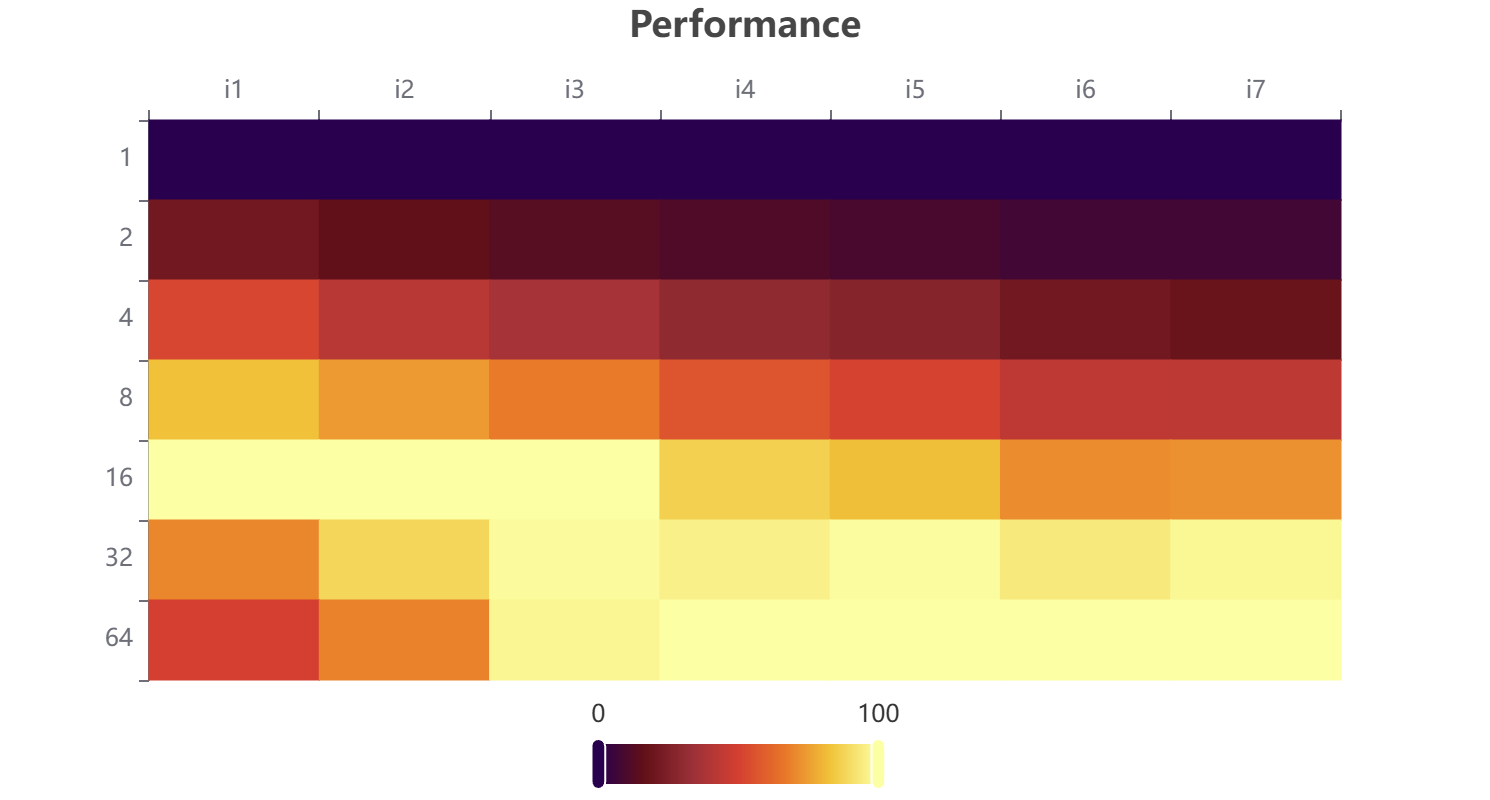
\includegraphics[width=\textwidth]{images/v1_barriers_Performance_Whole_Program_(Region_0).png}
\caption{v1, barreiras.}
\end{subfigure}\hfill
\begin{subfigure}{0.48\textwidth}\centering
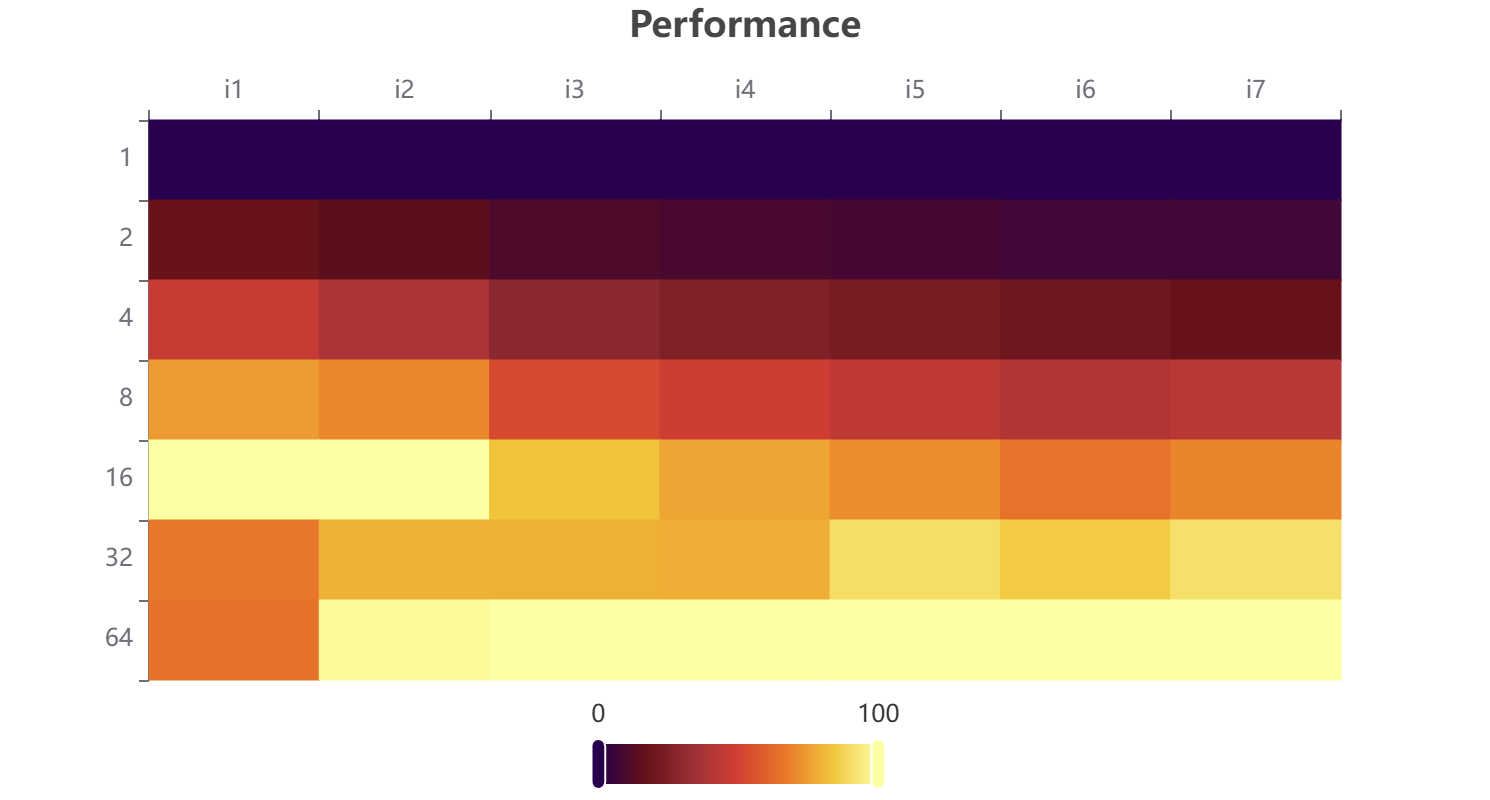
\includegraphics[width=\textwidth]{images/v2_private_Performance_Whole_Program_(Region_0).png}
\caption{v2, ponteiros privados.}
\end{subfigure}\\[0.6em]
\begin{subfigure}{0.48\textwidth}\centering
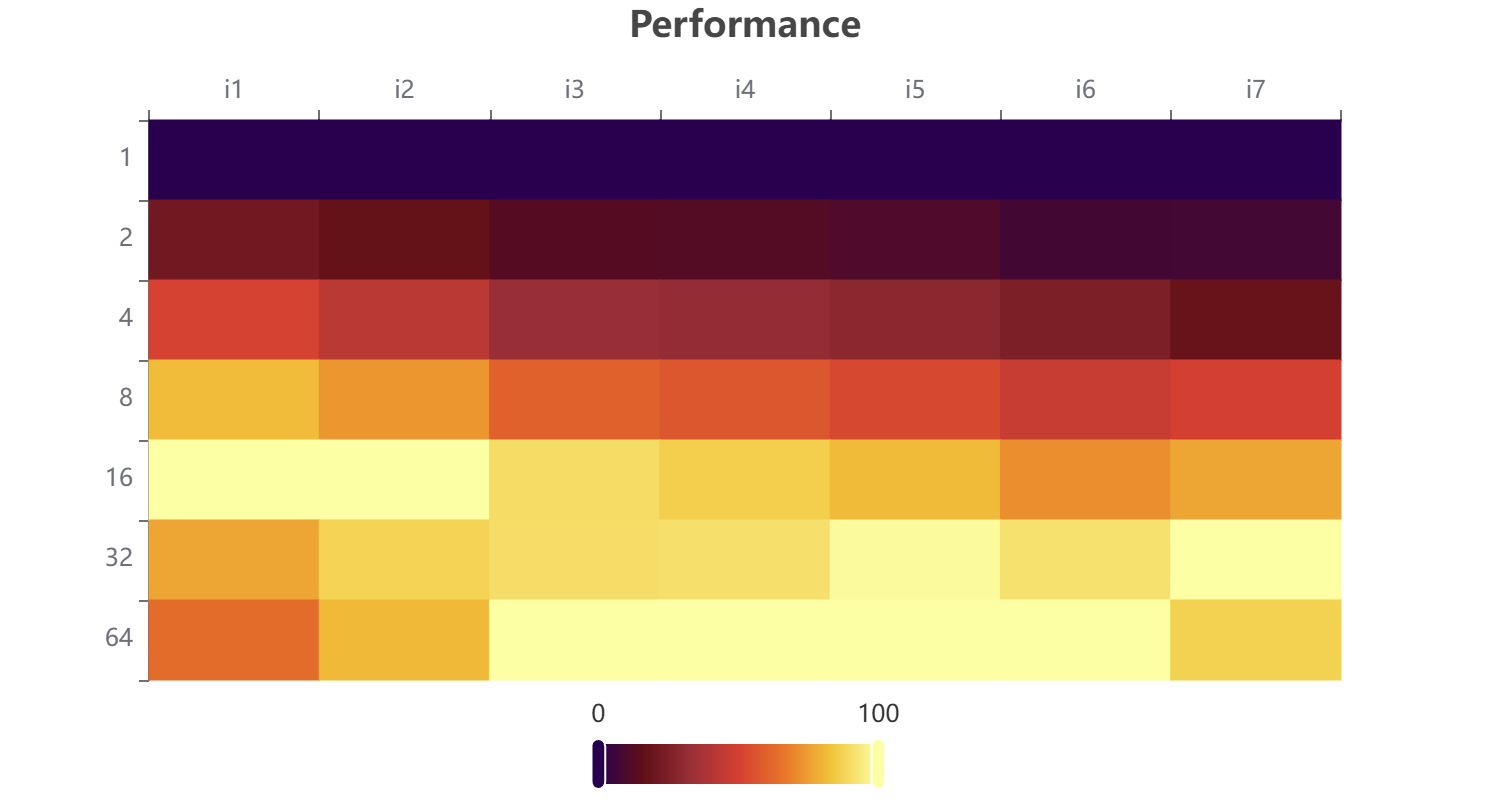
\includegraphics[width=\textwidth]{images/v3_simd_Performance_Whole_Program_(Region_0).png}
\caption{v3, SIMD.}
\end{subfigure}\hfill
\begin{subfigure}{0.48\textwidth}\centering
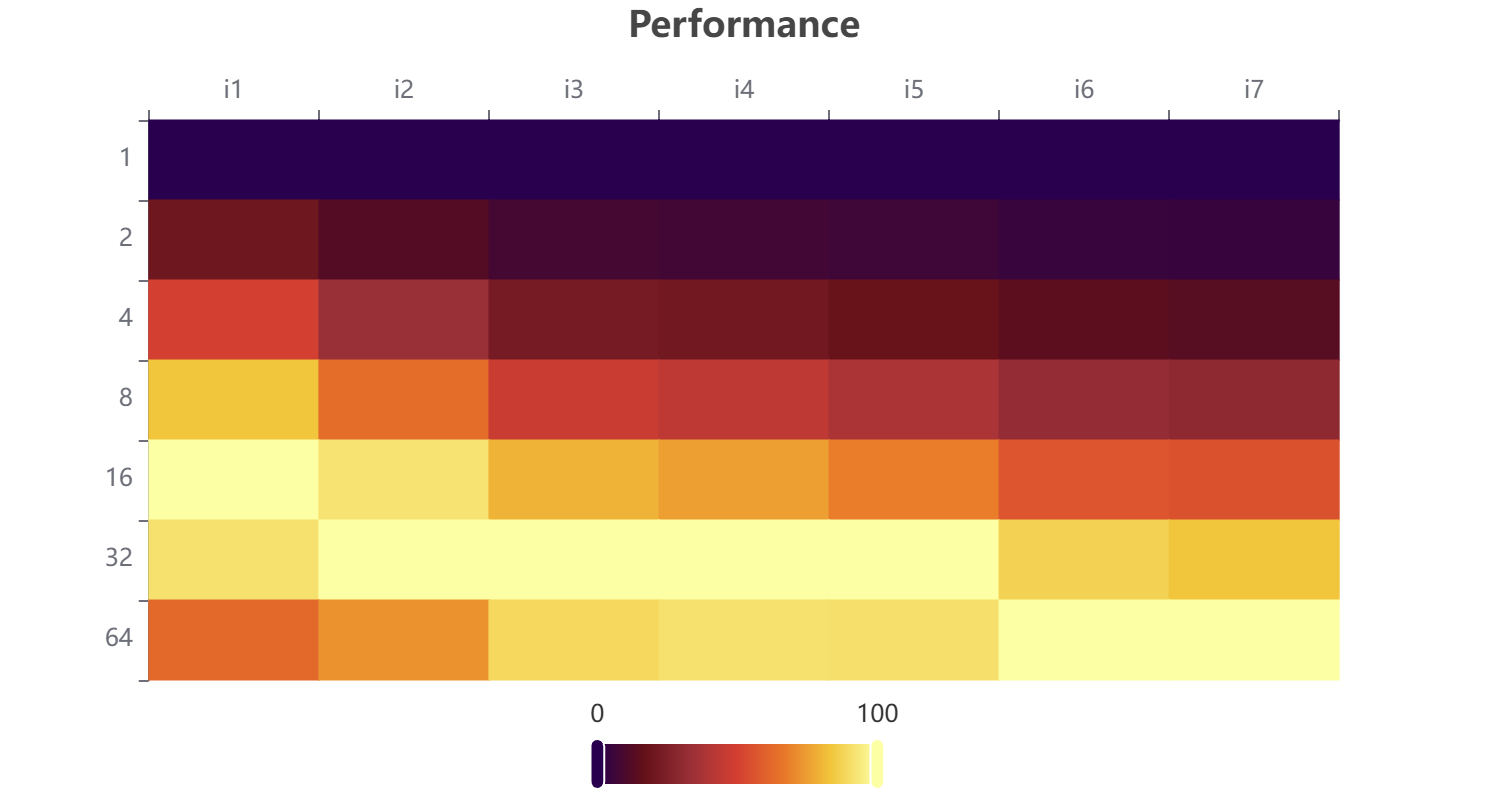
\includegraphics[width=\textwidth]{images/v4_numa_Performance_Whole_Program_(Region_0).png}
\caption{v4, inicialização paralela.}
\end{subfigure}
\caption{Desempenho do programa inteiro por versão. Linhas: threads. Colunas $i1$--$i7$: cargas crescentes.}
\label{fig:desempenho}
\end{figure}

\newpage
\subsection{Speedup}
O speedup do Viewer é próprio de cada versão, com referência em uma thread. Tons quentes marcam speedup maior dentro de cada figura. O crescimento acompanha o ideal linear apenas no início; com p maior, o overhead de sincronização por passo cresce junto e afasta a curva do ideal. Nas cargas grandes, o mesmo overhead representa fração menor do trabalho total, e o speedup se sustenta melhor. Ler cada coluna fixa equivale ao teste de escalabilidade forte.

\begin{figure}[H]\centering
\begin{subfigure}{0.48\textwidth}\centering
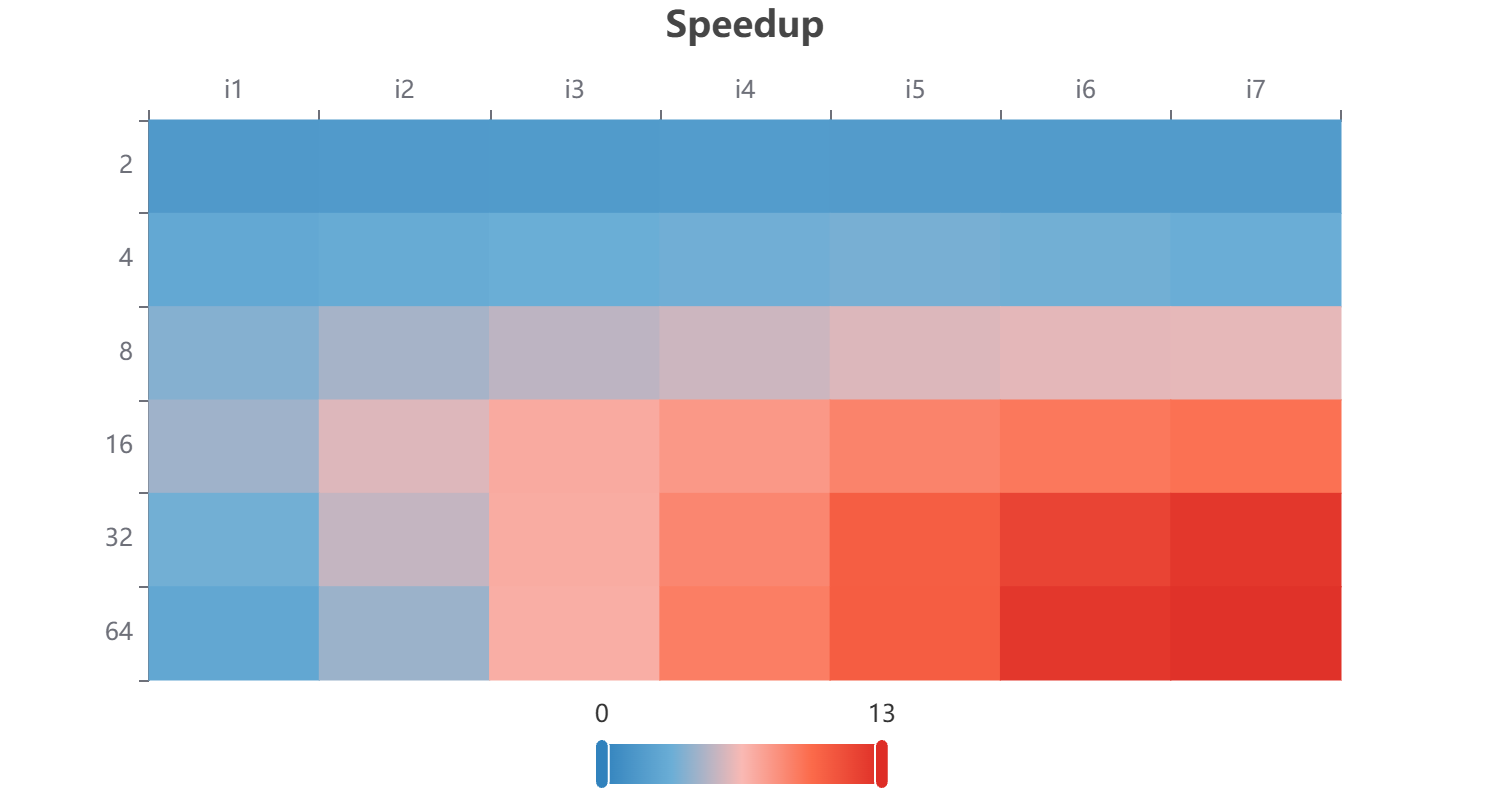
\includegraphics[width=\textwidth]{images/v1_barriers_Speedup_Whole_Program_(Region_0).png}
\caption{v1, barreiras.}
\end{subfigure}\hfill
\begin{subfigure}{0.48\textwidth}\centering
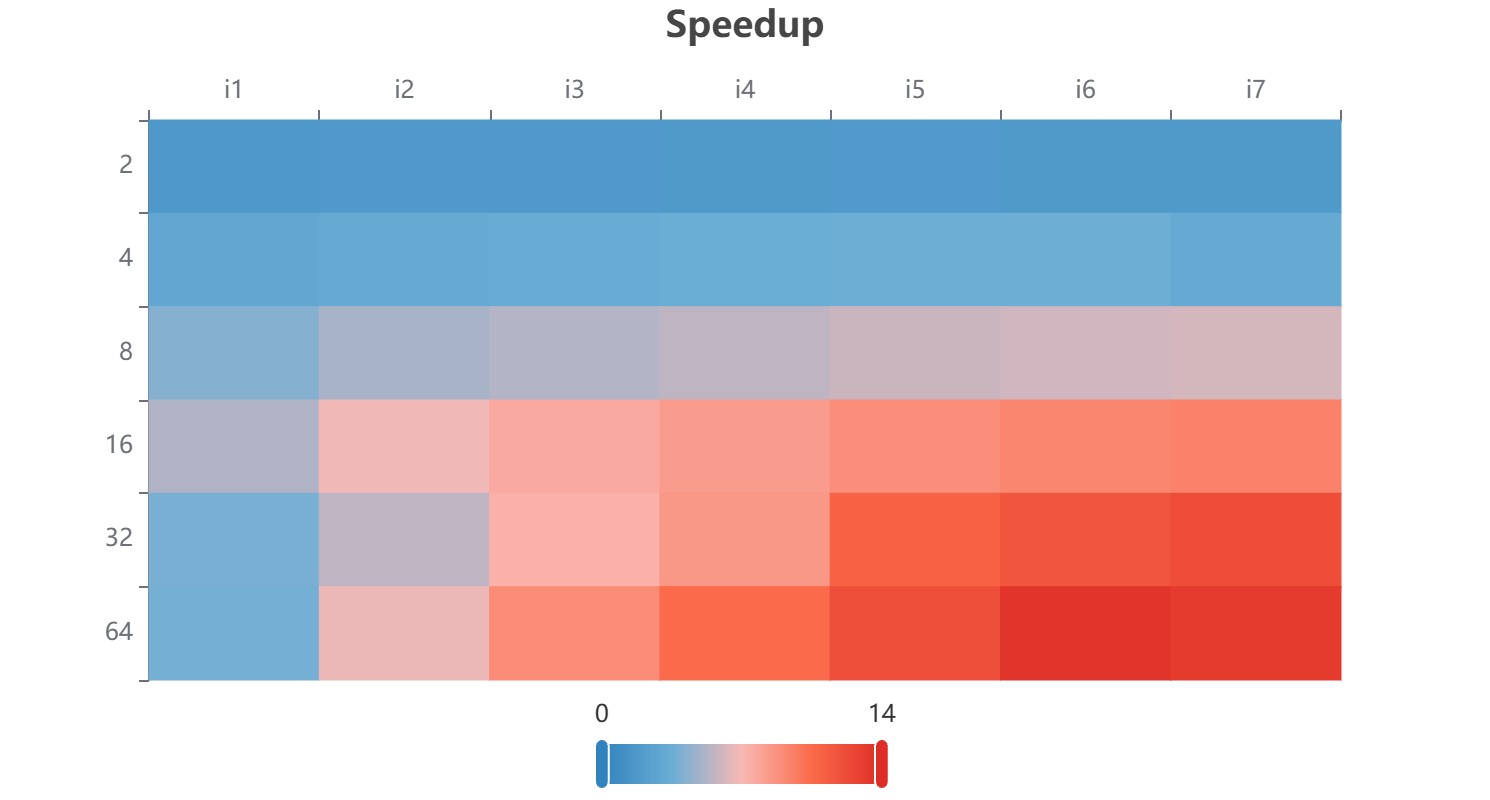
\includegraphics[width=\textwidth]{images/v2_private_Speedup_Whole_Program_(Region_0).png}
\caption{v2, ponteiros privados.}
\end{subfigure}\\[0.6em]
\begin{subfigure}{0.48\textwidth}\centering
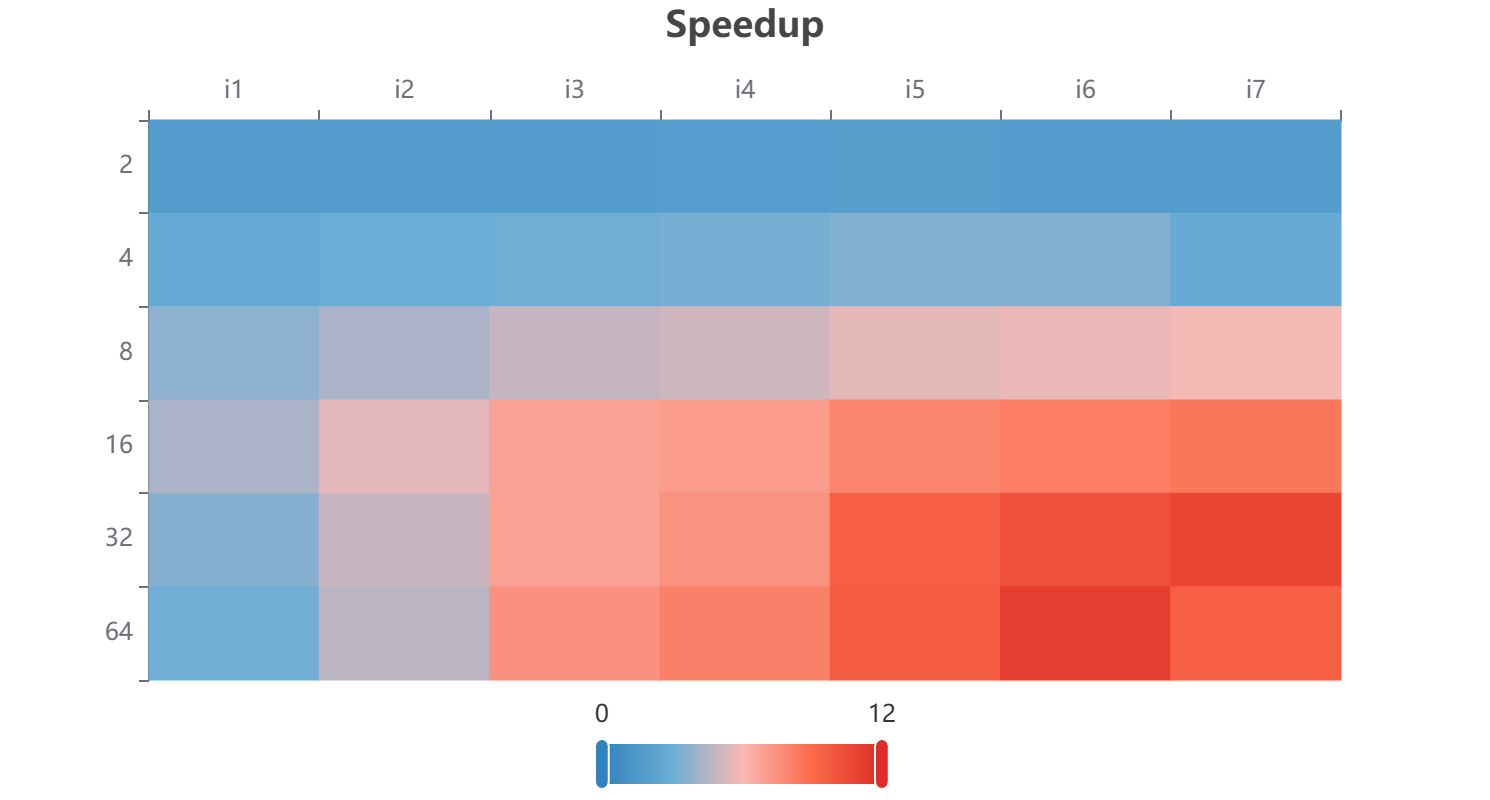
\includegraphics[width=\textwidth]{images/v3_simd_Speedup_Whole_Program_(Region_0).png}
\caption{v3, SIMD.}
\end{subfigure}\hfill
\begin{subfigure}{0.48\textwidth}\centering
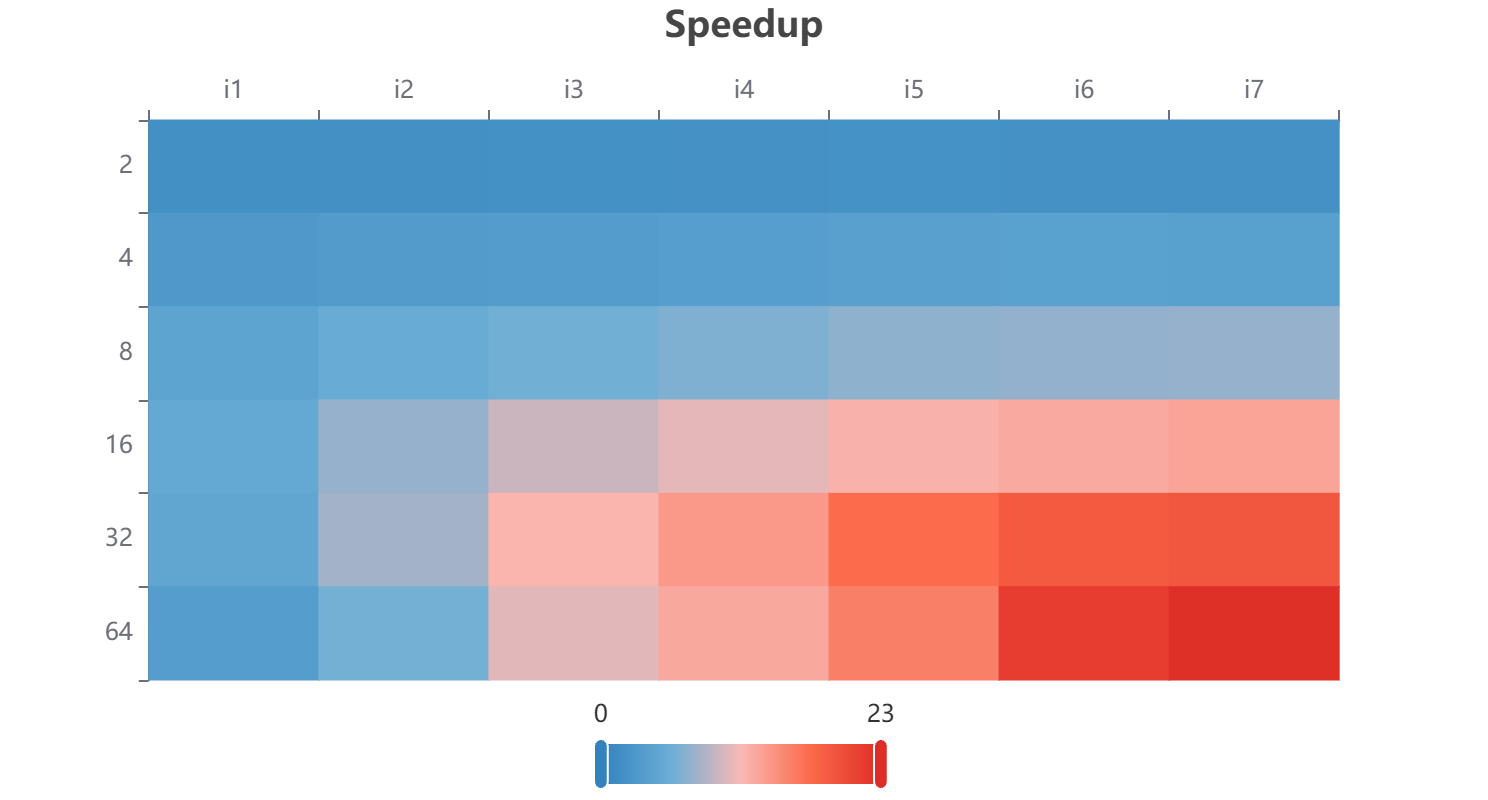
\includegraphics[width=\textwidth]{images/v4_numa_Speedup_Whole_Program_(Region_0).png}
\caption{v4, inicialização paralela.}
\end{subfigure}
\caption{Speedup próprio por versão. Linhas: threads. Colunas $i1$--$i7$: cargas crescentes.}
\label{fig:speedup}
\end{figure}

\newpage
\subsection{Eficiência}
A eficiência divide o speedup por $p$. Tons escuros marcam eficiência maior. Em trabalho fixo, a eficiência cai com $p$ em todas as versões e cargas: cada thread adicional acrescenta sincronização sem acrescentar trabalho. A queda acelera nas cargas pequenas, onde cada thread recebe poucas linhas e a parcela de coordenação domina a parcela útil.

\begin{figure}[H]\centering
\begin{subfigure}{0.48\textwidth}\centering
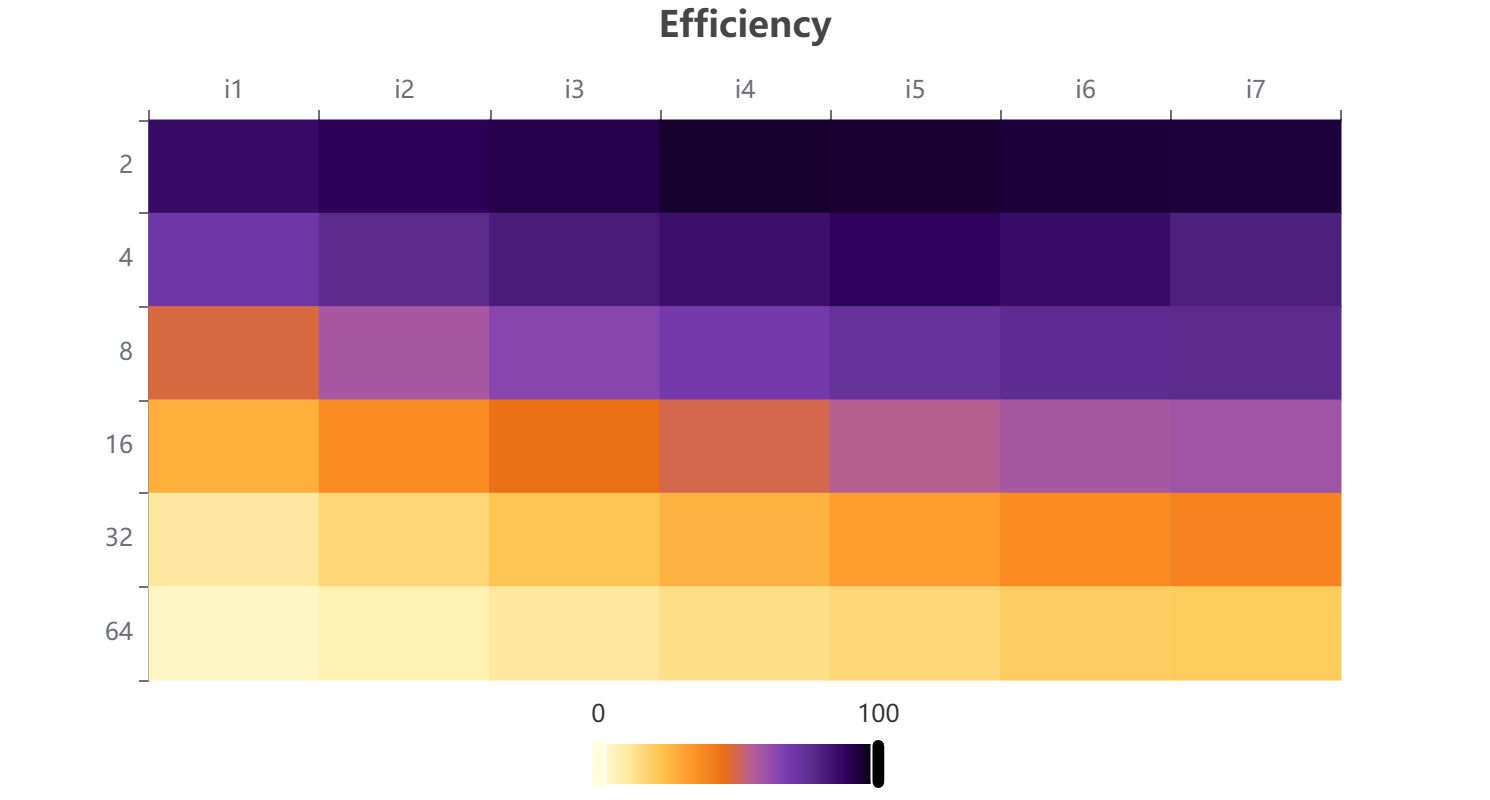
\includegraphics[width=\textwidth]{images/v1_barriers_Efficiency_Whole_Program_(Region_0).png}
\caption{v1, barreiras.}
\end{subfigure}\hfill
\begin{subfigure}{0.48\textwidth}\centering
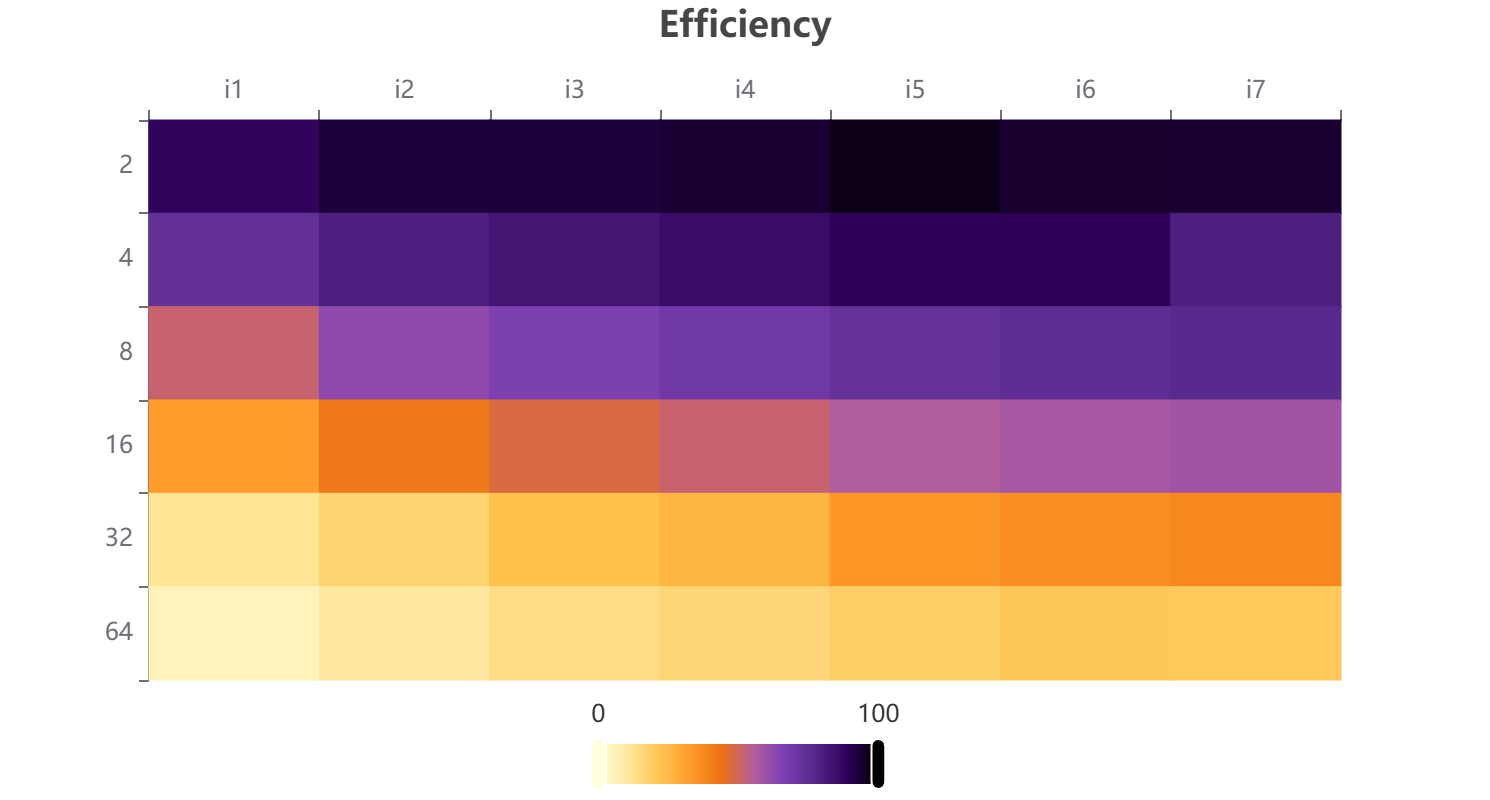
\includegraphics[width=\textwidth]{images/v2_private_Efficiency_Whole_Program_(Region_0).png}
\caption{v2, ponteiros privados.}
\end{subfigure}\\[0.6em]
\begin{subfigure}{0.48\textwidth}\centering
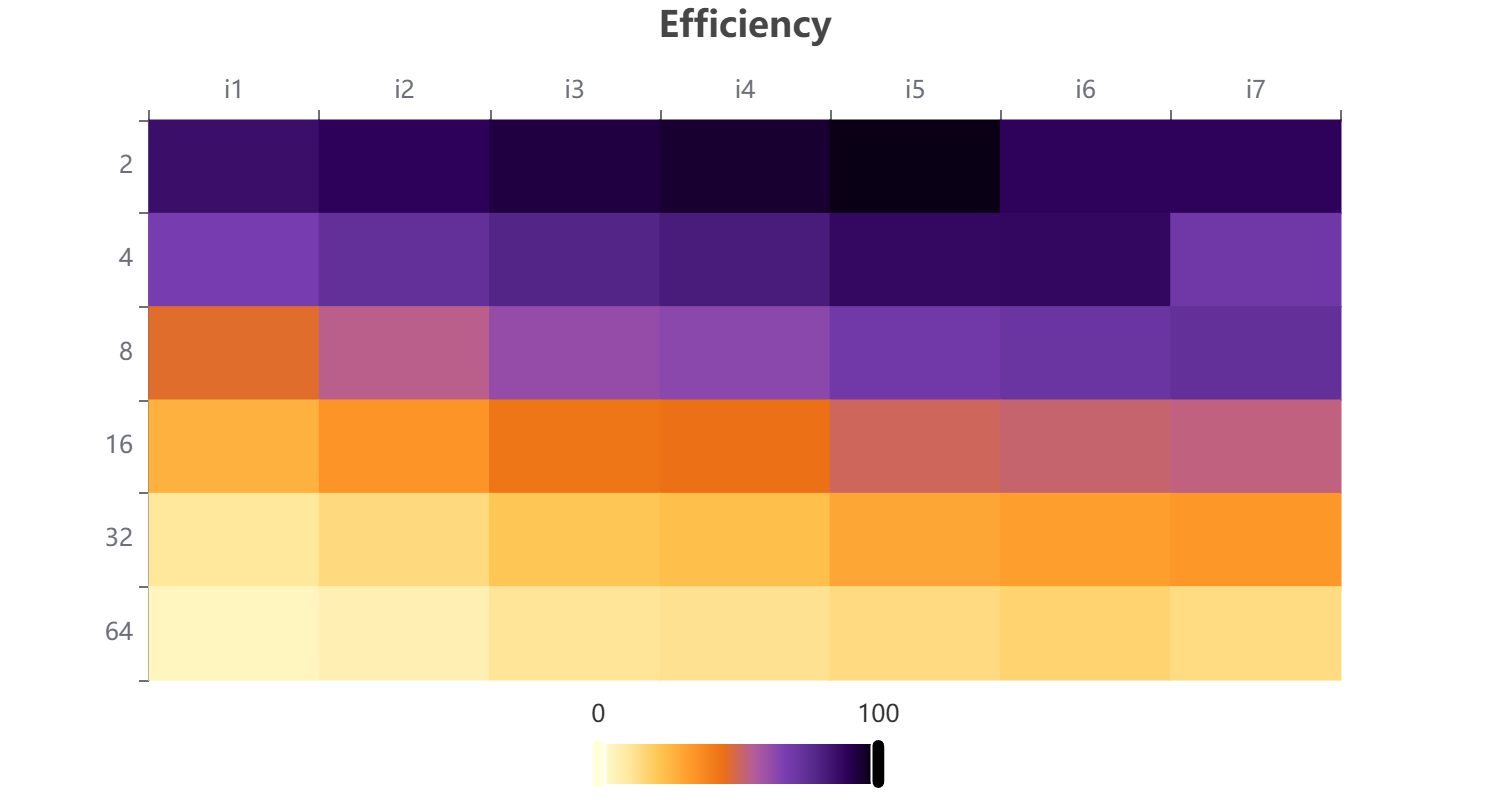
\includegraphics[width=\textwidth]{images/v3_simd_Efficiency_Whole_Program_(Region_0).png}
\caption{v3, SIMD.}
\end{subfigure}\hfill
\begin{subfigure}{0.48\textwidth}\centering
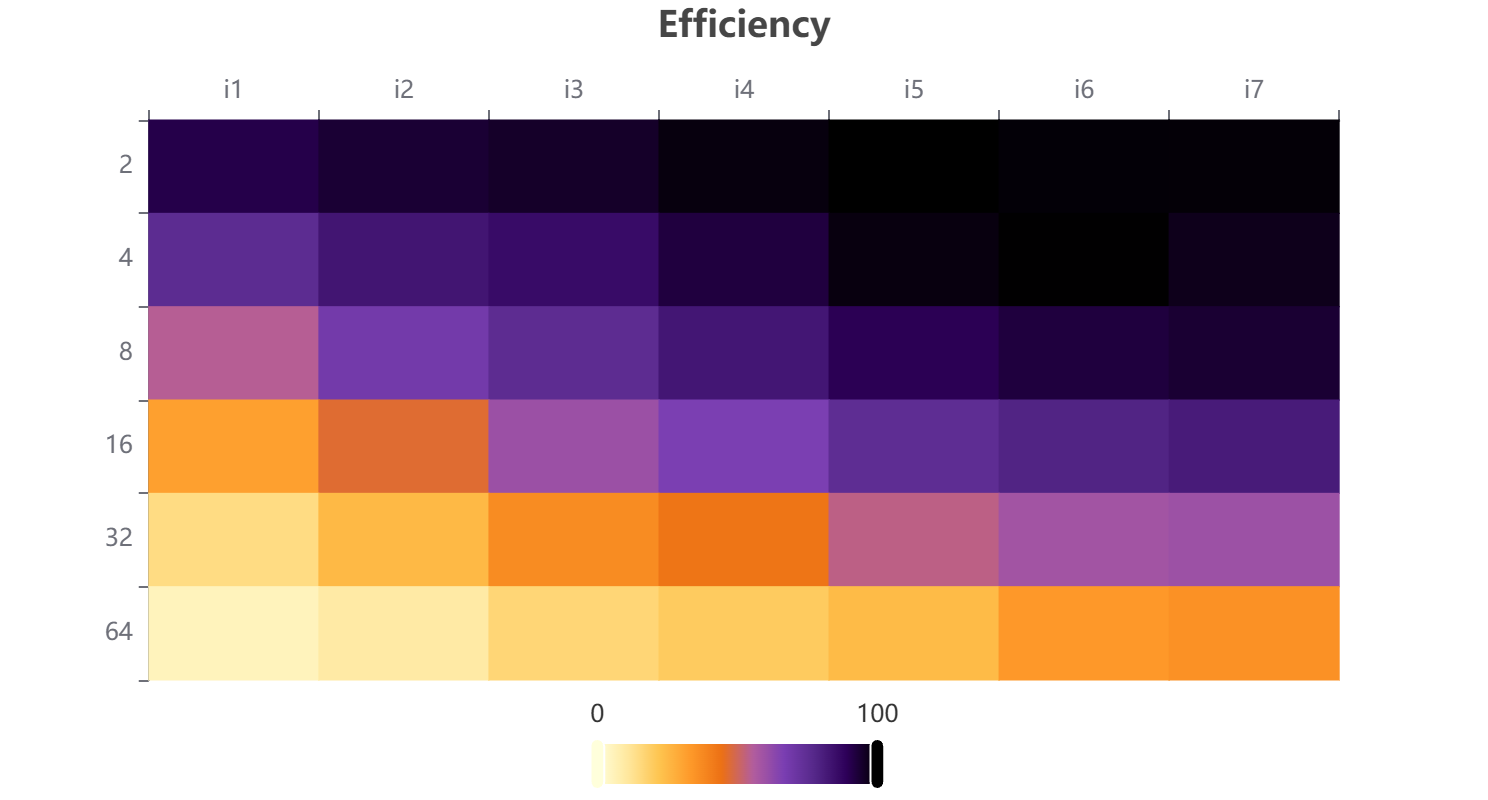
\includegraphics[width=\textwidth]{images/v4_numa_Efficiency_Whole_Program_(Region_0).png}
\caption{v4, inicialização paralela.}
\end{subfigure}
\caption{Eficiência por versão. Linhas: threads. Colunas $i1$--$i7$: cargas crescentes.}
\label{fig:eficiencia}
\end{figure}

\newpage
\subsection{Escalabilidade forte}
Cada coluna fixa a carga e varia as threads. O Viewer pinta quase tudo em tons de perda, piores em $p=32$ e $p=64$. A dependência temporal RAW entre passos exige uma barreira por passo em qualquer versão: são 500 sincronizações por execução, um custo de coordenação que não diminui quando p cresce. Com a carga fixa, cada thread recebe uma fatia cada vez mais fina do mesmo trabalho, e a coordenação passa a dominar. Nas fronteiras entre blocos, linhas de threads vizinhas podem dividir a mesma linha de cache e gerar tráfego de coerência, um mecanismo que cresce com p, mas os dados não o isolam. A célula isolada em $p=2$ e carga média destoa do entorno; com apenas uma repetição, indica variação, não ganho.

\begin{figure}[H]\centering
\begin{subfigure}{0.48\textwidth}\centering
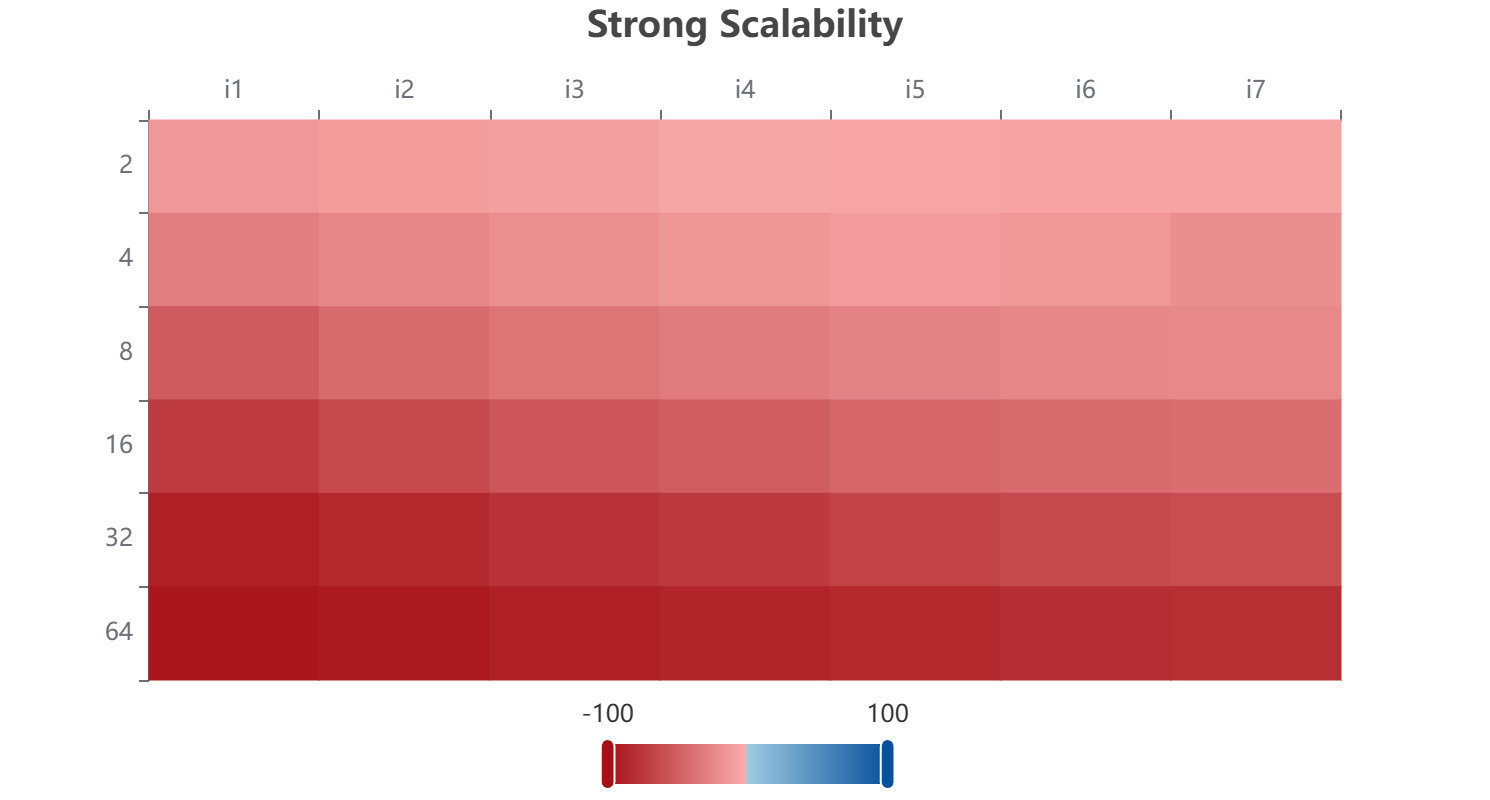
\includegraphics[width=\textwidth]{images/v1_barriers_Strong_Scalability_Whole_Program_(Region_0).png}
\caption{v1, barreiras.}
\end{subfigure}\hfill
\begin{subfigure}{0.48\textwidth}\centering
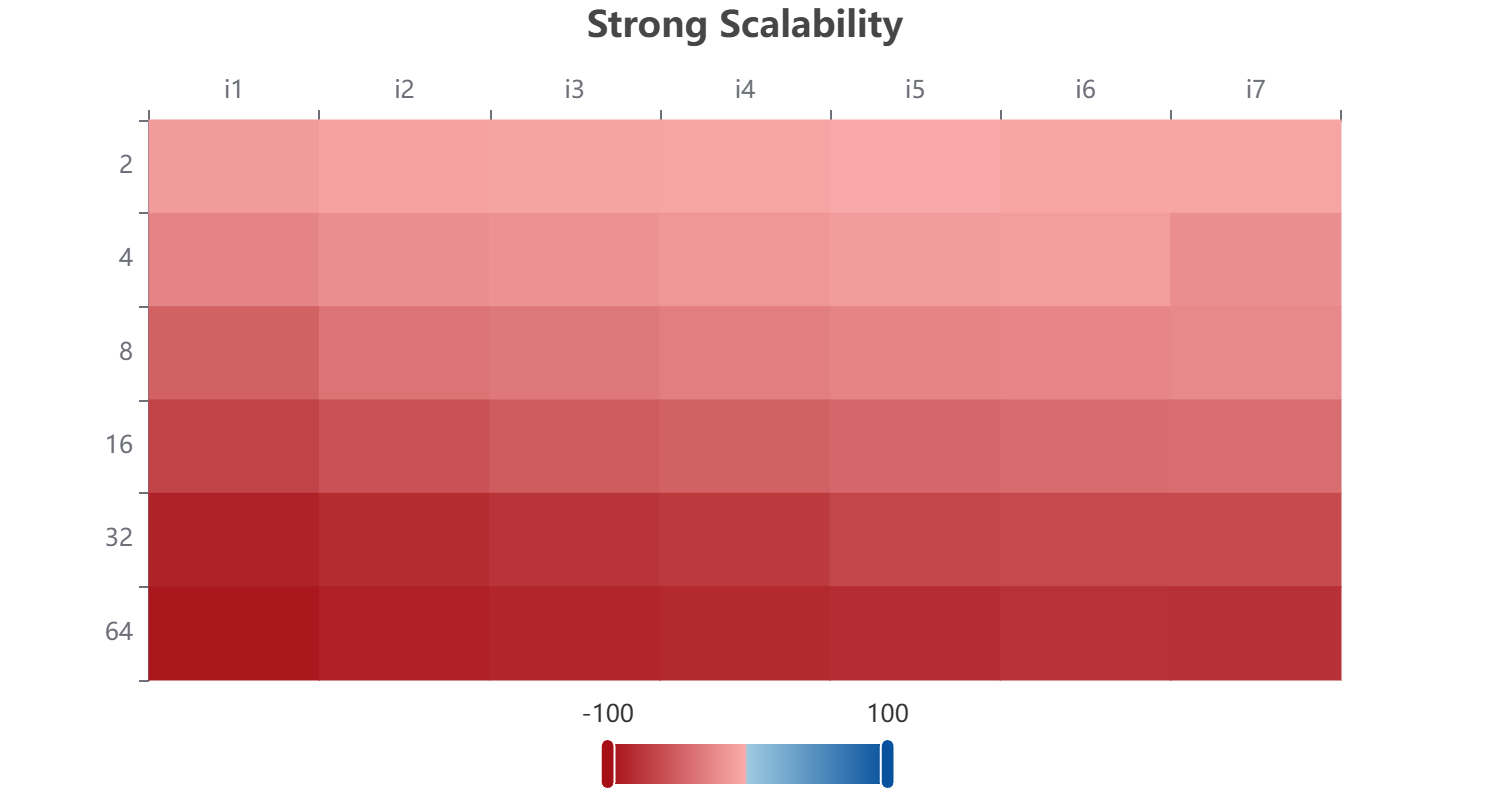
\includegraphics[width=\textwidth]{images/v2_private_Strong_Scalability_Whole_Program_(Region_0).png}
\caption{v2, ponteiros privados.}
\end{subfigure}\\[0.6em]
\begin{subfigure}{0.48\textwidth}\centering
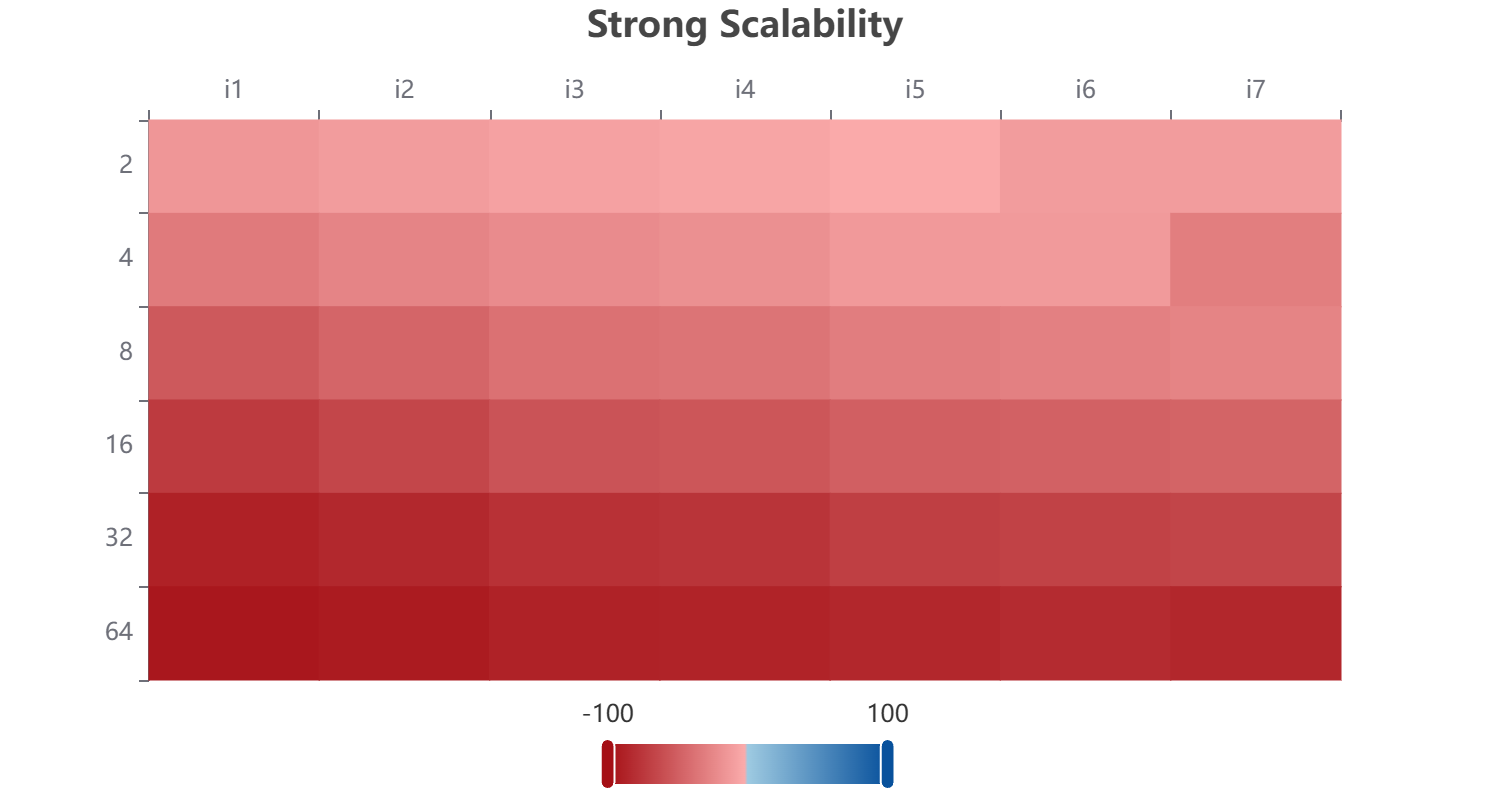
\includegraphics[width=\textwidth]{images/v3_simd_Strong_Scalability_Whole_Program_(Region_0).png}
\caption{v3, SIMD.}
\end{subfigure}\hfill
\begin{subfigure}{0.48\textwidth}\centering
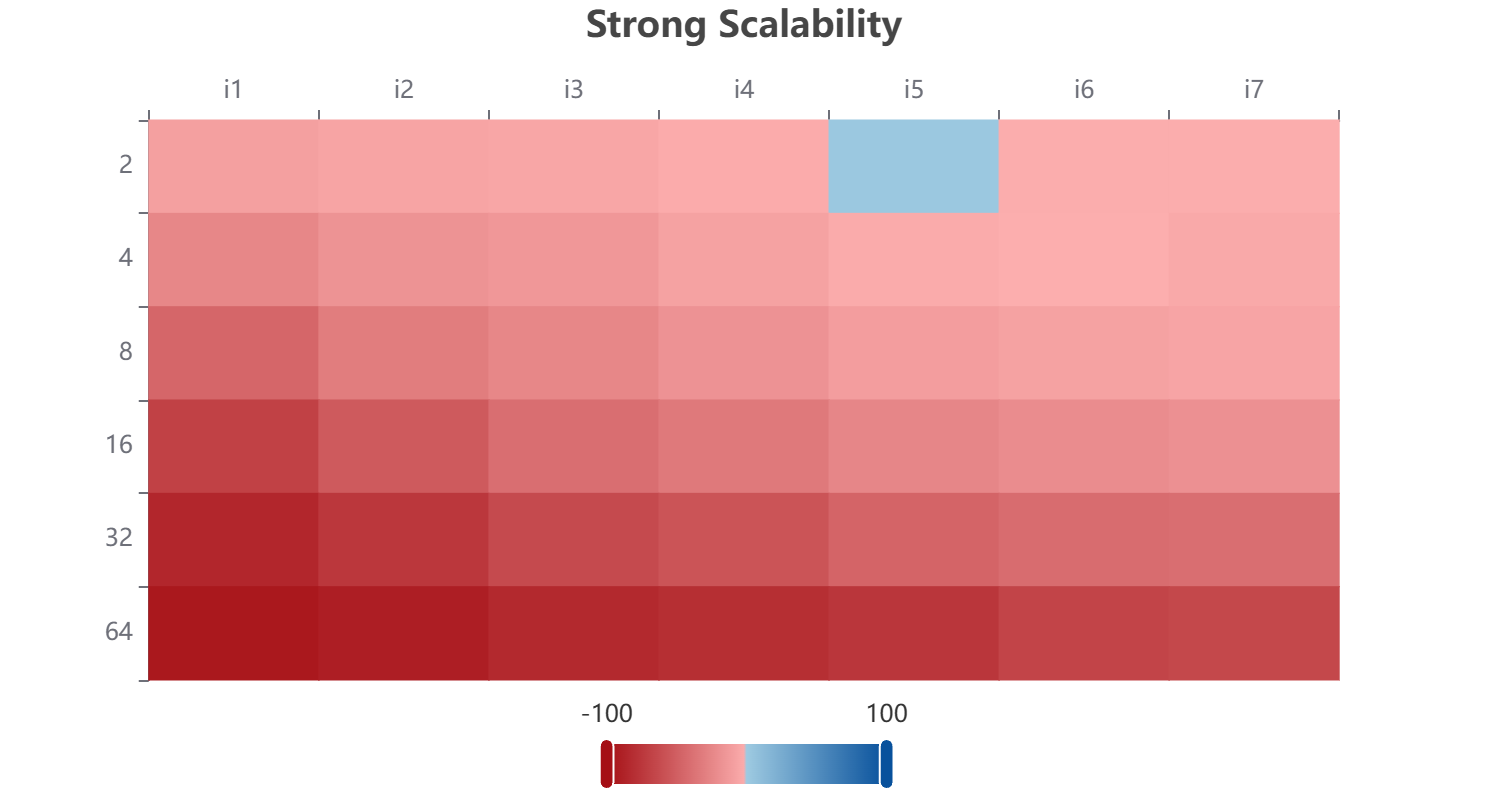
\includegraphics[width=\textwidth]{images/v4_numa_Strong_Scalability_Whole_Program_(Region_0).png}
\caption{v4, inicialização paralela.}
\end{subfigure}
\caption{Escalabilidade forte do programa inteiro. Linhas: threads. Colunas $i1$--$i7$: cargas fixas por coluna.}
\label{fig:forte}
\end{figure}

\newpage
\subsection{Escalabilidade fraca}
A diagonal mantém a carga por thread quase constante. Há escalabilidade fraca quando a eficiência se preserva ao aumentar problema e threads na mesma proporção. O Viewer pinta a diagonal na mesma faixa de perda das outras células, pior em $p=64$: nessa faixa, dobrar carga e threads não preservou a eficiência. Duas ressalvas limitam a leitura. Primeiro, a região do programa inteiro inclui a parcela serial de alocação e inicialização, que impõe um teto à maneira de Amdahl sobre qualquer indicador medido no total. Segundo, a célula isolada em $p=2$ reaparece aqui e indica variação, não ganho. O teste usual de carga constante por thread exige repetições e a região de evolução separada.

\begin{figure}[H]\centering
\begin{subfigure}{0.48\textwidth}\centering
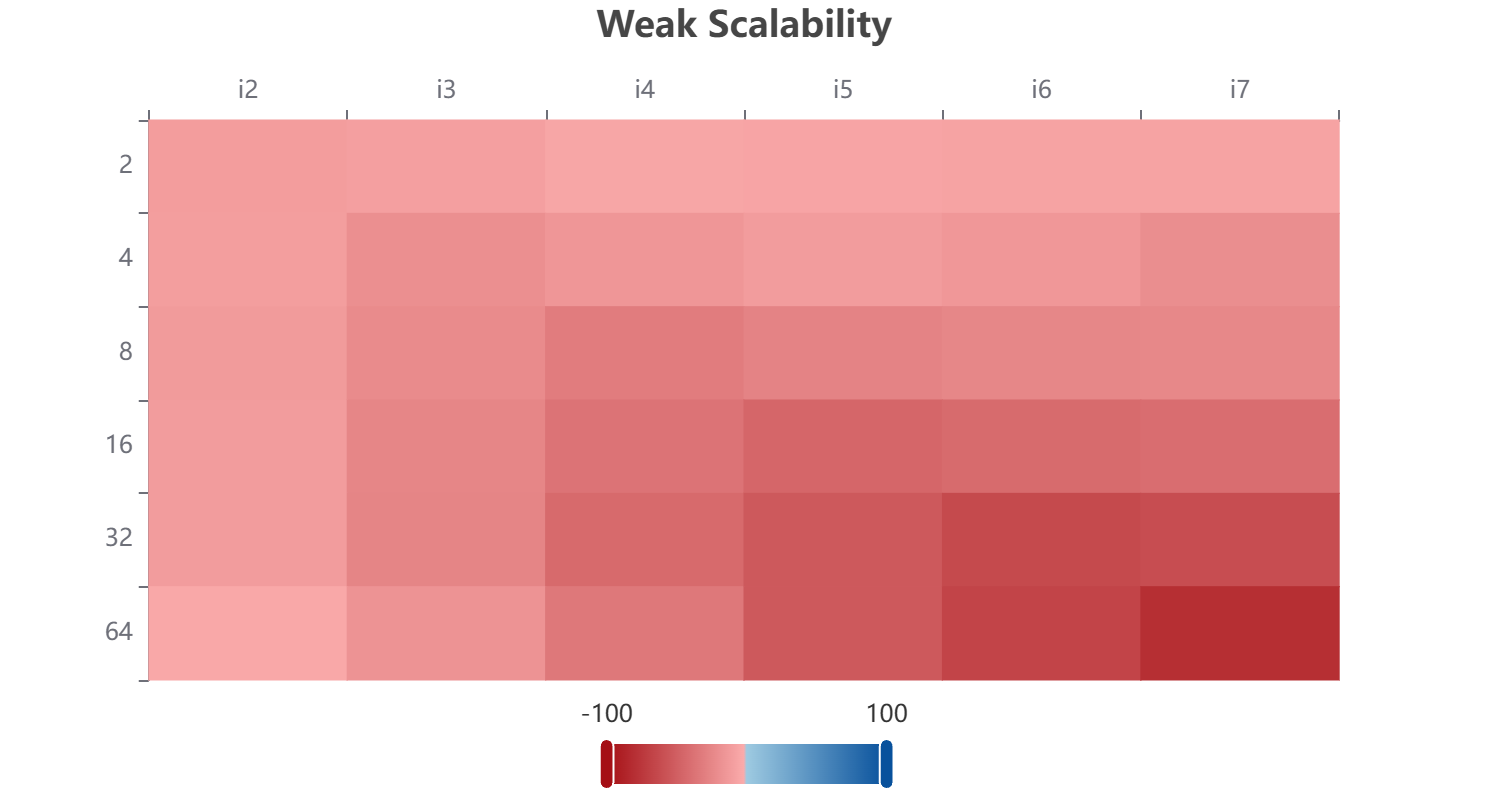
\includegraphics[width=\textwidth]{images/v1_barriers_Weak_Scalability_Whole_Program_(Region_0).png}
\caption{v1, barreiras.}
\end{subfigure}\hfill
\begin{subfigure}{0.48\textwidth}\centering
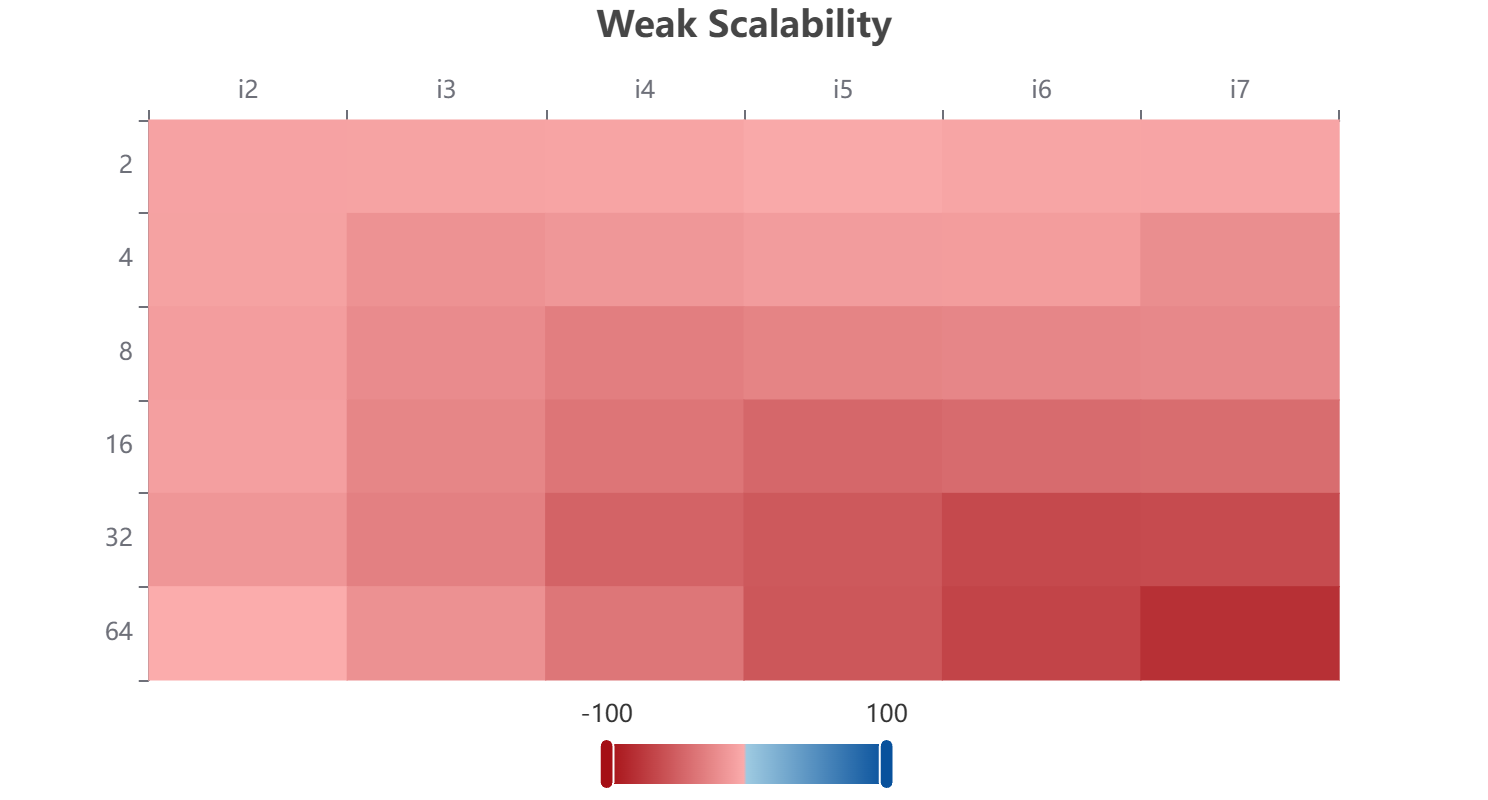
\includegraphics[width=\textwidth]{images/v2_private_Weak_Scalability_Whole_Program_(Region_0).png}
\caption{v2, ponteiros privados.}
\end{subfigure}\\[0.6em]
\begin{subfigure}{0.48\textwidth}\centering
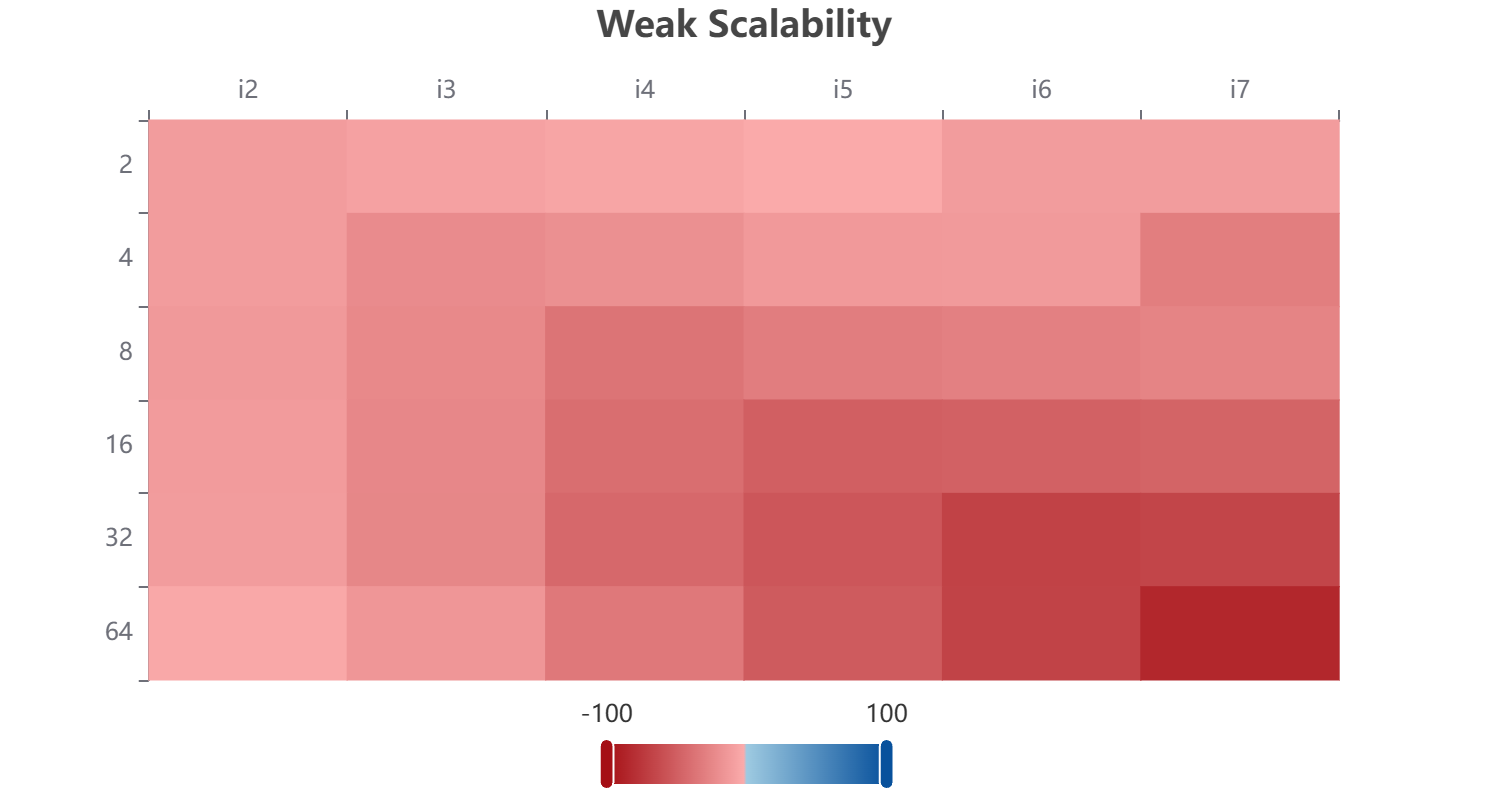
\includegraphics[width=\textwidth]{images/v3_simd_Weak_Scalability_Whole_Program_(Region_0).png}
\caption{v3, SIMD.}
\end{subfigure}\hfill
\begin{subfigure}{0.48\textwidth}\centering
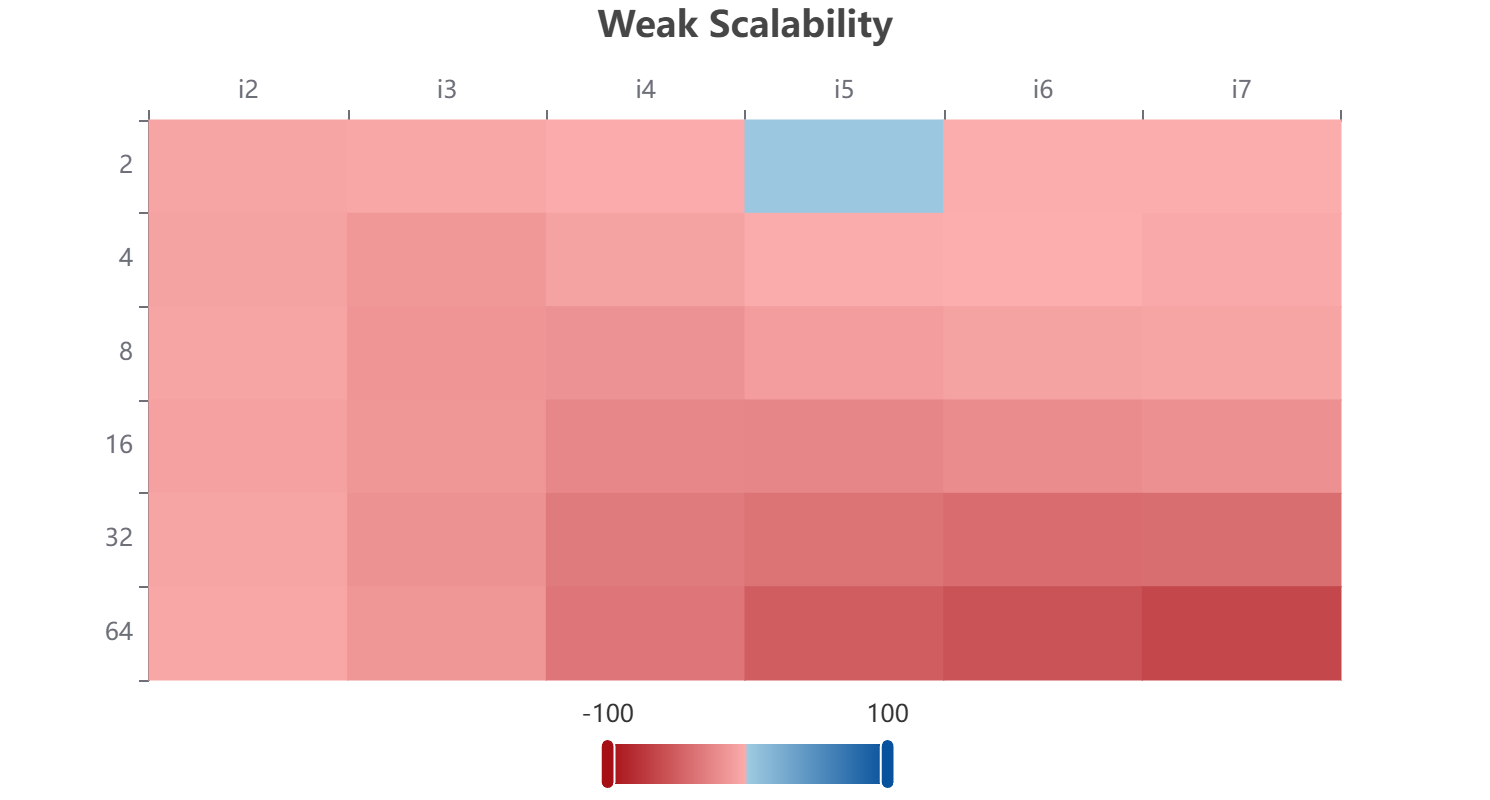
\includegraphics[width=\textwidth]{images/v4_numa_Weak_Scalability_Whole_Program_(Region_0).png}
\caption{v4, inicialização paralela.}
\end{subfigure}
\caption{Escalabilidade fraca do programa inteiro. Linhas: threads. Colunas $i2$--$i7$: cargas da diagonal.}
\label{fig:fraca}
\end{figure}

\newpage
\subsection{Escalabilidade geral}
O diagrama geral combina trabalho e recursos. Um programa é escalável, no sentido formal, quando existe um ritmo de crescimento do problema que preserva a eficiência à medida que p aumenta. As quatro versões ficam em faixa intermediária, com o melhor relativo em $p=8$ e $p=16$ nas cargas médias e piora em $p=64$. A eficiência se segura só no meio da faixa. Fora dali, overhead, barreiras e granularidade fina mandam. A figura cobre o programa inteiro, sem separar inicialização de evolução.

\begin{figure}[H]\centering
\begin{subfigure}{0.48\textwidth}\centering
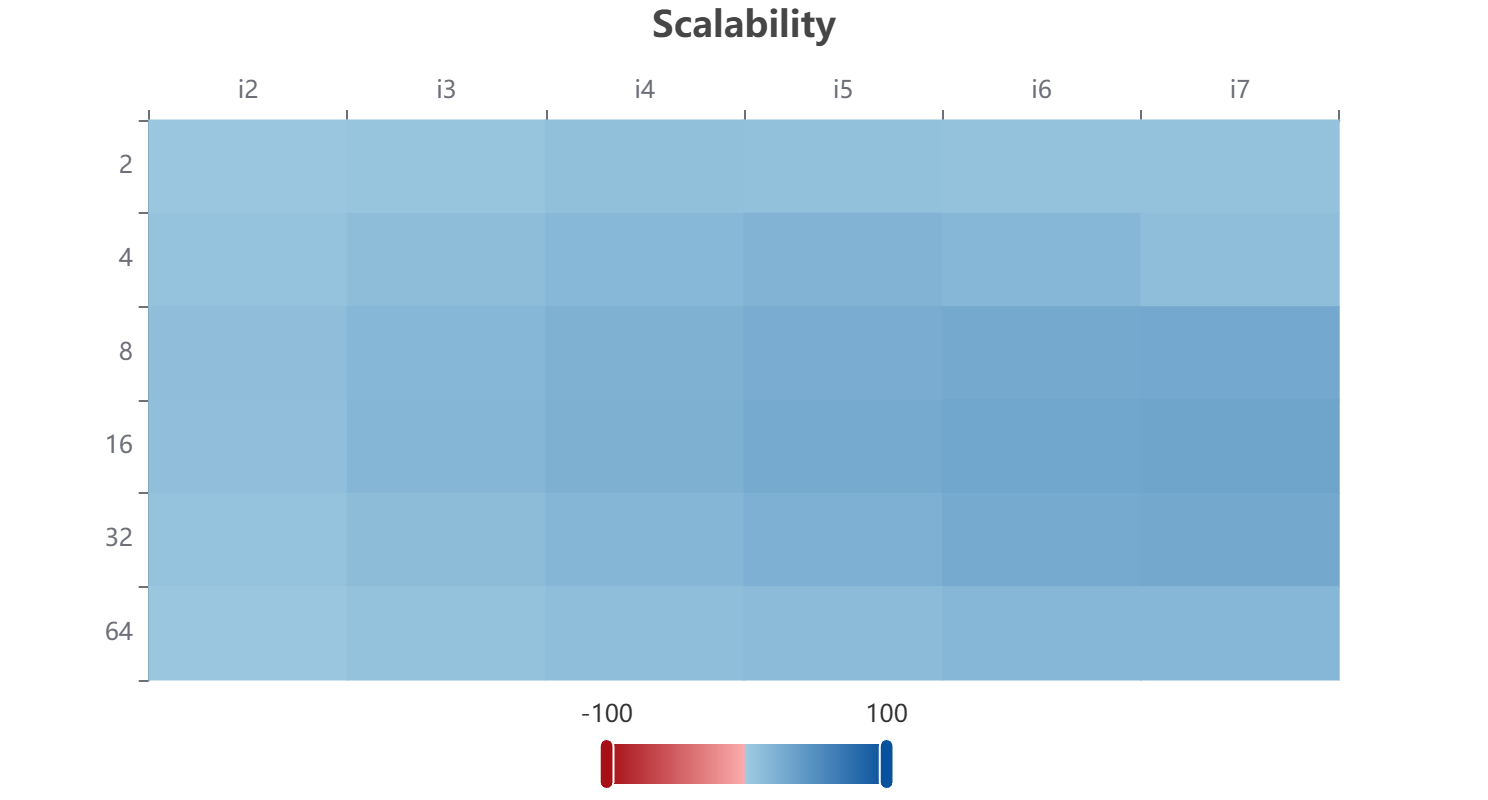
\includegraphics[width=\textwidth]{images/v1_barriers_Scalability_Whole_Program_(Region_0).png}
\caption{v1, barreiras.}
\end{subfigure}\hfill
\begin{subfigure}{0.48\textwidth}\centering
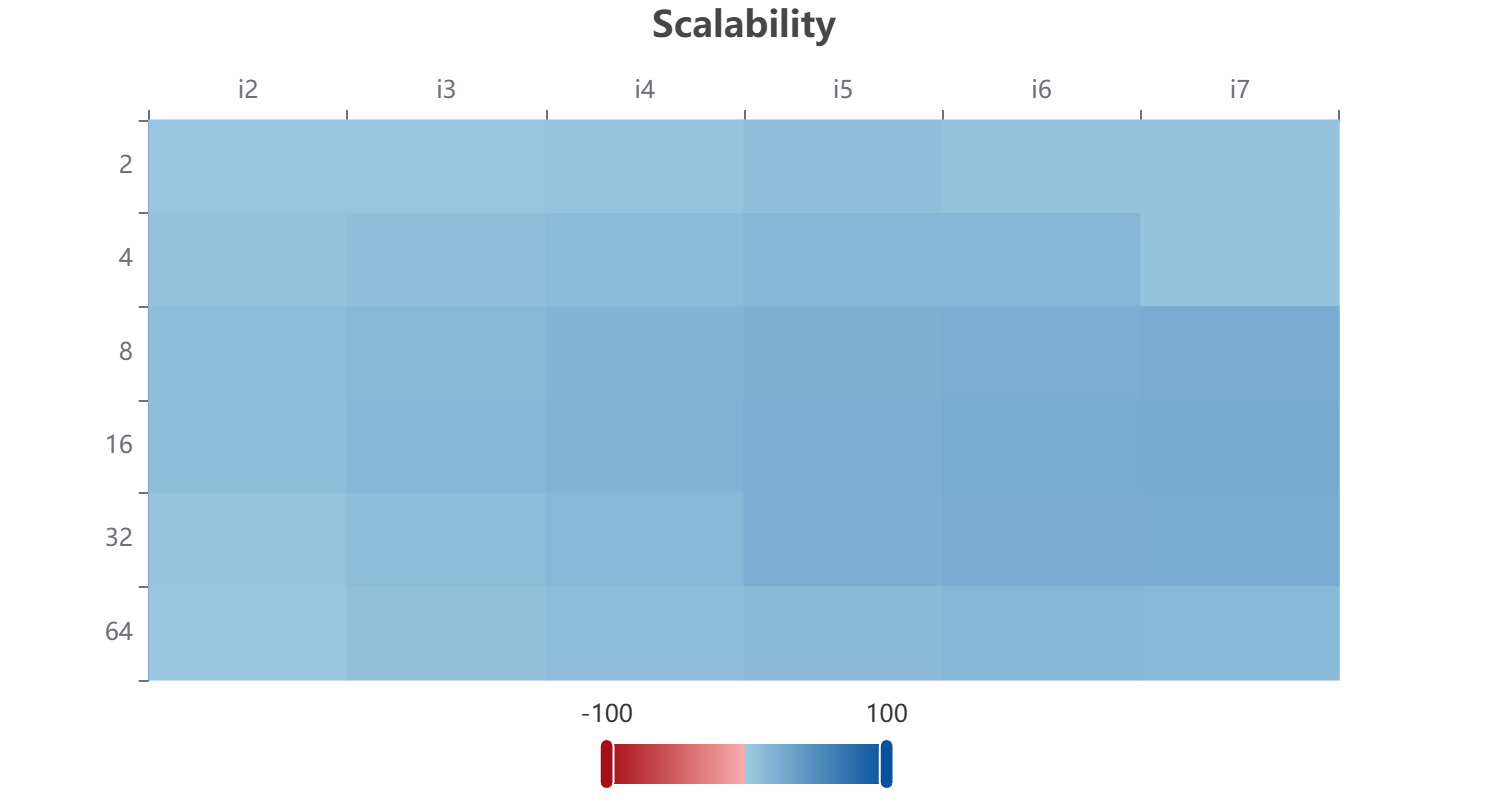
\includegraphics[width=\textwidth]{images/v2_private_Scalability_Whole_Program_(Region_0).png}
\caption{v2, ponteiros privados.}
\end{subfigure}\\[0.6em]
\begin{subfigure}{0.48\textwidth}\centering
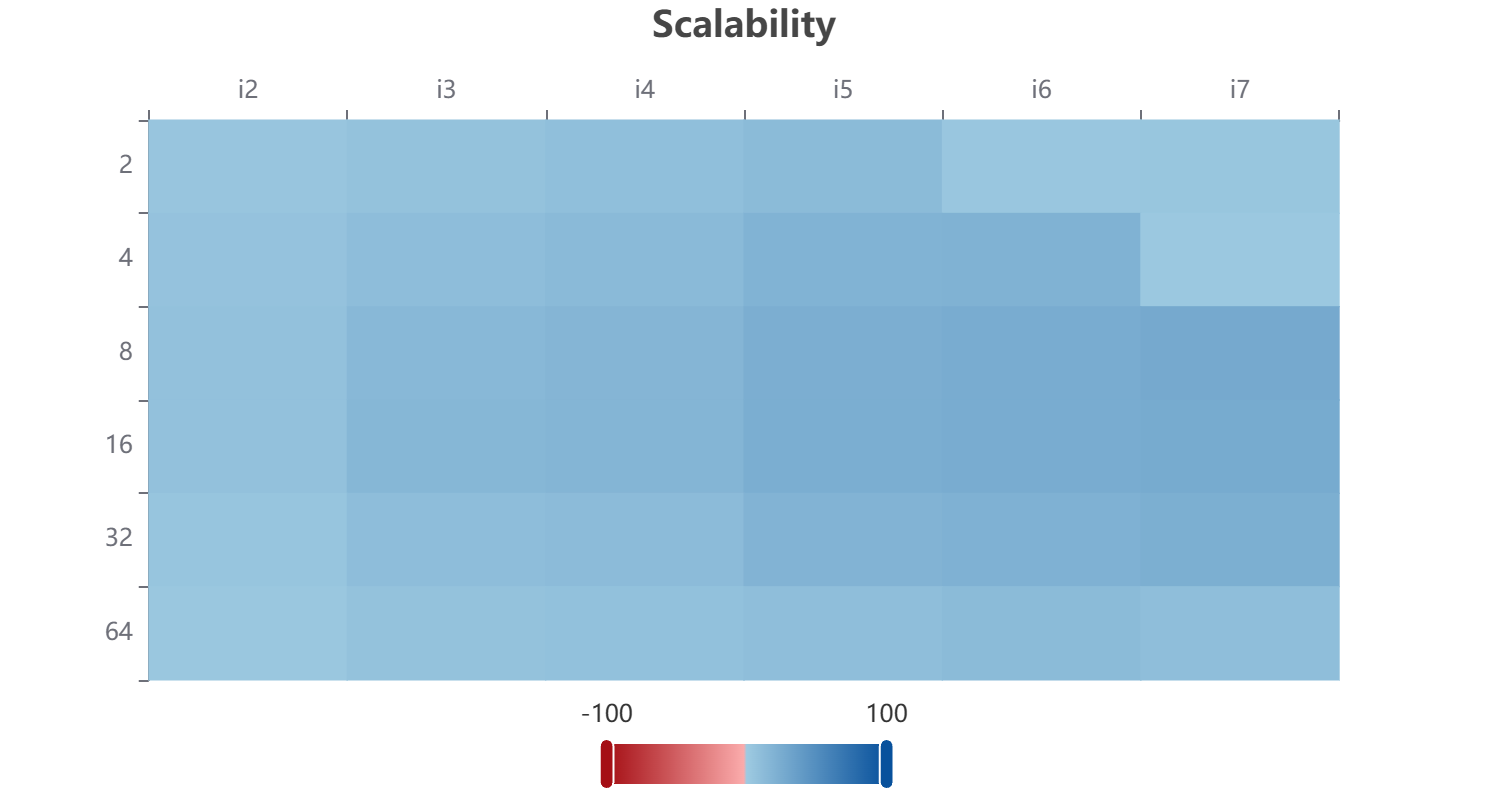
\includegraphics[width=\textwidth]{images/v3_simd_Scalability_Whole_Program_(Region_0).png}
\caption{v3, SIMD.}
\end{subfigure}\hfill
\begin{subfigure}{0.48\textwidth}\centering
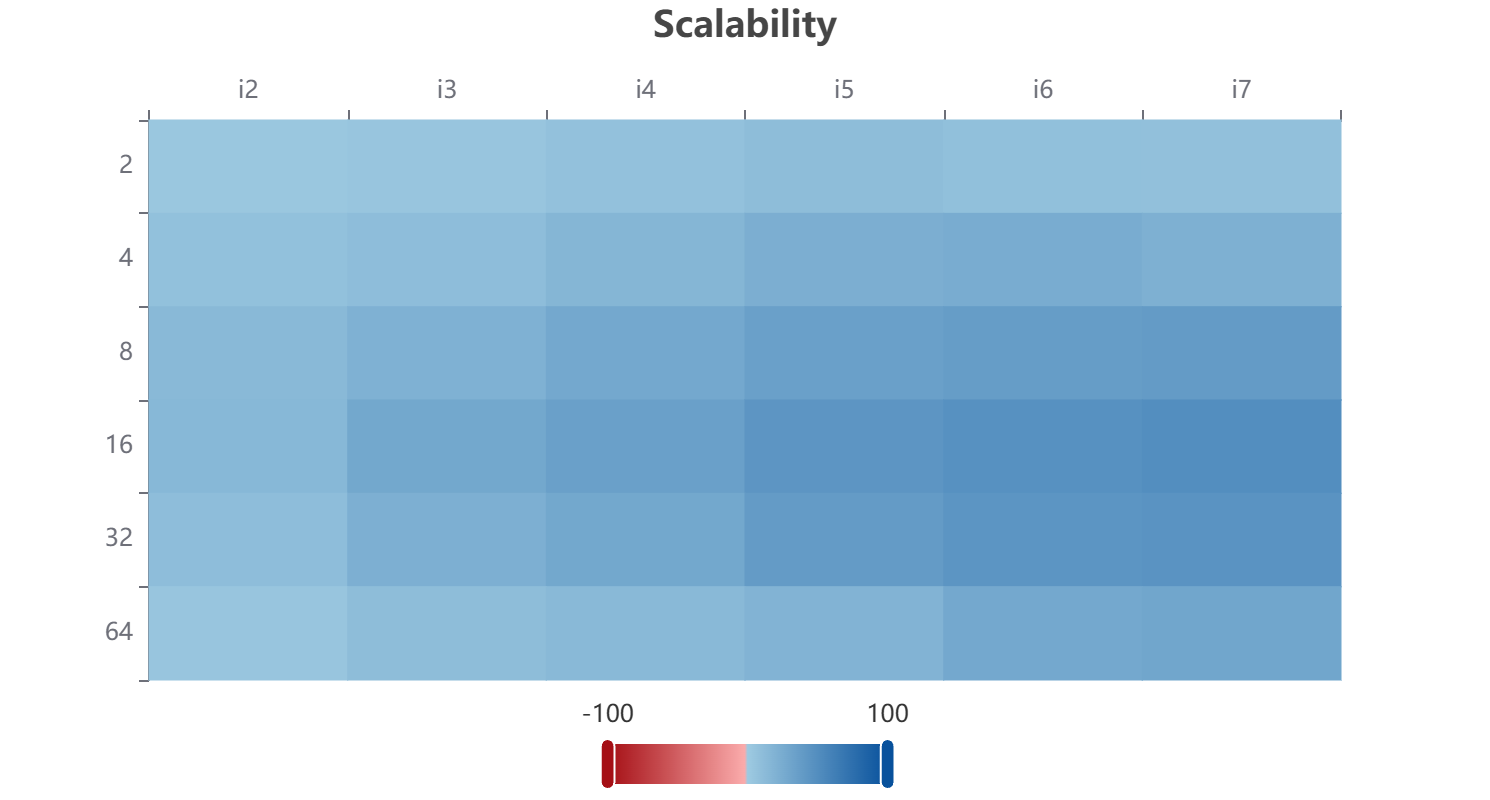
\includegraphics[width=\textwidth]{images/v4_numa_Scalability_Whole_Program_(Region_0).png}
\caption{v4, inicialização paralela.}
\end{subfigure}
\caption{Escalabilidade geral do programa inteiro. Linhas: threads. Colunas $i2$--$i7$.}
\label{fig:geral}
\end{figure}

\newpage
\subsection{Comparação entre versões}
\begin{table}[H]\centering\small
\begin{tabular}{p{2.4cm}p{4.0cm}p{4.0cm}p{4.0cm}}\hline
Transição & O que muda & Efeito esperado & Observado\\\hline
Barreiras $\to$ ponteiros privados & Sai a barreira do \texttt{single}; ficam trabalho por thread, \texttt{static} e a barreira do \texttt{omp for} (RAW). & Menos 500 sincronizações por execução. & Mesmo padrão nos mapas; sem evolução separada, o ganho não se distingue.\\
Ponteiros privados $\to$ SIMD & Entra \texttt{omp simd} no laço interno. & Vetorização explícita do laço de células. & Sem relatório de vetorização, sem efeito visível; o compilador pode já vetorizar sozinho.\\
SIMD $\to$ inicialização paralela & A escrita inicial dos dois campos passa ao laço distribuído. & Menor fração serial e first touch distribuído. & Sem evolução separada e sem dados de páginas, sem atribuição a NUMA.\\\hline
\end{tabular}
\caption{Transições entre estratégias: mudança, efeito esperado e observado.}
\label{tab:transicoes}
\end{table}

\appendix\newpage
\section{Código-fonte}
Os arquivos \texttt{v1\_barriers.c} (barreiras), \texttt{v2\_private.c} (ponteiros privados), \texttt{v3\_simd.c} (SIMD) e \texttt{v4\_numa.c} (inicialização paralela) compartilham \texttt{main()}, medição com \texttt{omp\_get\_wtime()}, exportação e a aritmética do stencil. A atualização executada em cada célula é a mesma nas quatro versões:
\begin{lstlisting}[caption={Núcleo comum do stencil.}]
size_t c = (size_t)i*n+j;
v[c] = u[c] + r * (u[c-1]+u[c+1]+u[c-n]+u[c+n]-4*u[c]);
\end{lstlisting}
Da estratégia com barreiras para a de ponteiros privados, a troca compartilhada dá lugar à troca local:
\begin{lstlisting}[caption={v1: troca em single, segunda barreira do passo.}]
#pragma omp single
{ double *tmp = u; u = v; v = tmp; }
\end{lstlisting}
\begin{lstlisting}[caption={v2: ponteiros privados e troca local.}]
double *a = u, *b = v; /* Ponteiros privados; campos compartilhados. */
/* Lacos espaciais e stencil identicos. */
double *tmp = a; a = b; b = tmp; /* Troca local, sem single. */
return steps % 2 ? v : u;
\end{lstlisting}
Da de ponteiros privados para SIMD, entra uma única linha no laço interno:
\begin{lstlisting}[caption={v3: acréscimo sobre v2.}]
#pragma omp simd
\end{lstlisting}
Da SIMD para inicialização paralela, a cópia serial dá lugar à escrita distribuída:
\begin{lstlisting}[caption={v3 e anteriores: inicialização serial.}]
memcpy(v, u, count * sizeof(*v));
\end{lstlisting}
\begin{lstlisting}[caption={v4: inicialização distribuída.}]
#pragma omp parallel for schedule(static) default(none) shared(u,v,n,mode)
/* Mesmo preenchimento, nos dois campos. */
v[c] = u[c];
\end{lstlisting}
\end{document}
